%\documentclass{beamer}
\documentclass[handout]{beamer}
\usetheme{Marburg}
\useoutertheme{infolines}
\newcommand{\answers}{1}

\usepackage{amsmath}
\usepackage{caption}
\usepackage{color}
\usepackage{enumerate}
\usepackage{listings}
\usepackage{hyperref}
\usepackage{mathrsfs}
\usepackage{natbib}
\usepackage{url}

\providecommand{\all}{\ \forall \ }
\providecommand{\bs}{\backslash}
\providecommand{\e}{\varepsilon}
\providecommand{\E}{\ \exists \ }
\providecommand{\lm}[2]{\lim_{#1 \rightarrow #2}}
\providecommand{\m}[1]{\mathbb{#1}}
\providecommand{\nv}{{}^{-1}}
\providecommand{\ov}[1]{\overline{#1}}
\providecommand{\p}{\newpage}
\providecommand{\q}{$\quad$ \newline}
\providecommand{\rt}{\rightarrow}
\providecommand{\Rt}{\Rightarrow}
\providecommand{\vc}[1]{\boldsymbol{#1}}
\providecommand{\wh}[1]{\widehat{#1}}

\hypersetup{colorlinks,linkcolor=,urlcolor=blue}
\numberwithin{equation}{section}

\definecolor{dkgreen}{rgb}{0,0.6,0}
\definecolor{gray}{rgb}{0.5,0.5,0.5}
\definecolor{mauve}{rgb}{0.58,0,0.82}

\lstset{ 
  language=C,                % the language of the code
  basicstyle= \footnotesize,           % the size of the fonts that are used for the code
  numbers=left,
  numberfirstline=true,
  numbersep=5pt,                  % how far the line-numbers are from the code
  backgroundcolor=\color{white},      % choose the background color. You must add \usepackage{color}
  showspaces=false,               % show spaces adding particular underscores
  showstringspaces=false,         % underline spaces within strings
  showtabs=false,                 % show tabs within strings adding particular underscores
  frame=lrb,                   % adds a frame around the code
  rulecolor=\color{black},        % if not set, the frame-color may be changed on line-breaks within not-black text 
  tabsize=2,                      % sets default tabsize to 2 spaces
  captionpos=t,                   % sets the caption-position 
  breaklines=true,                % sets automatic line breaking
  breakatwhitespace=false,        % sets if automatic breaks should only happen at whitespace
  %title=\lstname,                   % show the filename of files included with \lstinputlisting;
  keywordstyle=\color{blue},          % keyword style
  commentstyle=\color{gray},       % comment style
  stringstyle=\color{dkgreen},         % string literal style
  escapeinside={\%*}{*)},            % if you want to add LaTeX within your code
  morekeywords={*, ...},               % if you want to add more keywords to the set
  xleftmargin=0.2in, % left horizontal offset of caption box
  xrightmargin=-.03in % right horizontal offset of caption box
}

%\DeclareCaptionFont{white}{\color{white}}
%\DeclareCaptionFormat{listing}{\parbox{\textwidth}{\colorbox{gray}{\parbox{\textwidth}{#1#2#3}}\vskip-0.05in}}
%\captionsetup[lstlisting]{format = listing, labelfont = white, textfont = white}
%For caption-free listings, comment out the 3 lines above and uncomment the 2 lines below.
 \captionsetup{labelformat = empty, labelsep = none}
 \lstset{frame = single}

\title{Introduction to programming in CUDA C}
\author{Will Landau}
\date{September 30, 2013}
\institute{Iowa State University}

\begin{document}

\begin{frame}
\titlepage
 \end{frame}
 
 \begin{frame}
\frametitle{Outline}
\tableofcontents
\end{frame}
 
 \AtBeginSection[]
{
   \begin{frame}
       \frametitle{Outline}
       \tableofcontents[currentsection]
   \end{frame}
}

\section{A review: GPU parallelism and CUDA architecture}

\begin{frame}[fragile]
\frametitle{The single instruction, multiple data (SIMD) paradigm}

\begin{itemize}
\pause \item SIMD: apply the same command to multiple places in a dataset. 

\pause \begin{lstlisting}
for(i = 0; i < 1e6; ++i)
  a[i] = b[i] + c[i];
\end{lstlisting}


\pause \item On CPUs, the iterations of the loop run sequentially.

\pause \item With GPUs, we can easily run all 1,000,000 iterations simultaneously.

\pause \begin{lstlisting}
i = threadIdx.x;
a[i] = b[i] + c[i];
\end{lstlisting}

\pause \item We can similarly \emph{parallelize} a lot more than just loops.
\end{itemize}
\end{frame}


\begin{frame}
\frametitle{CPU / GPU cooperation}

\begin{itemize}
\item The CPU (``host") is in charge.
\uncover<2->{\item The CPU sends computationally intensive instruction sets to the GPU (``device") just like a human uses a pocket calculator.}
\end{itemize}

\begin{center}
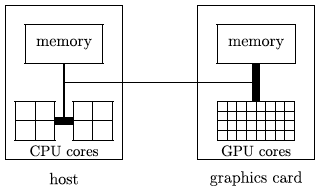
\includegraphics[scale=.8]{../../fig/communication.png}
\end{center}
\end{frame}


\begin{frame}
\frametitle{How GPU parallelism works}
\begin{enumerate}
\item The CPU sends a command called a {\bf kernel} to a GPU.
\pause \item The GPU executes several duplicate realizations of this command, called {\bf threads}.
\begin{itemize}
\pause \item These threads are grouped into bunches called {\bf blocks}.
\pause \item The sum total of all threads in a kernel is called a {\bf grid}.
\end{itemize}
\end{enumerate}

\begin{itemize}
\item Toy example:
\begin{itemize}
\item CPU says: ``Hey, GPU. Sum pairs of adjacent numbers. Use the array, (1, 2, 3, 4, 5, 6, 7, 8)."
\pause \item GPU thinks: ``Sum pairs of adjacent numbers" is a kernel.
\pause \item The GPU spawns 2 blocks, each with 2 threads:
\end{itemize}
\end{itemize}

\pause \begin{center}
\begin{tabular}{c|cc|cc}
Block  & \multicolumn{2}{c|}{0} &  \multicolumn{2}{c}{1} \\ \hline
Thread & 0 & 1 & 0 & 1  \\ \hline
Action & 1 + 2 & 3 + 4 & 5 + 6 & 7 + 8 \\
\end{tabular}
\end{center}

\begin{itemize}
\pause \item I could have also used 1 block with 4 threads and given the threads different pairs of numbers.
\end{itemize}
\end{frame}

\begin{frame}
\begin{center}
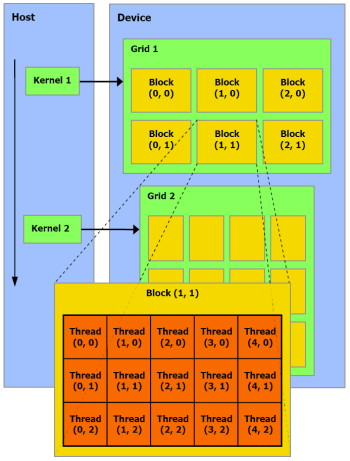
\includegraphics[scale=.7]{../../fig/gridBlocksThreads.jpg}
\end{center}
\end{frame}

\begin{frame}
\frametitle{CUDA: making a gaming toy do science}
\begin{itemize}
\pause \item {\bf CUDA}: Compute Unified Device Architecture. 
\pause \item Before CUDA, programmers could only do GPU programming in graphics languages, which are appropriate for video games but clumsy for science.
\pause \item CUDA devices support CUDA C, an extension of C for programs that use GPUs.
\pause \item CUDA-enabled servers at Iowa State:
\begin{itemize}
\item impact1.stat.iastate.edu
\item impact2.stat.iastate.edu 
\item impact3.stat.iastate.edu 
\item impact4.stat.iastate.edu (in the works...)
\end{itemize}
\end{itemize}
\end{frame}

\section{Beginning CUDA C}

\subsection{Hello world}

\begin{frame}[fragile]
\frametitle{Hello world}

\small

\begin{itemize}
\item A beginner C program:
\end{itemize}

\lstset{basicstyle=\scriptsize}

\begin{lstlisting}
#include <stdio.h> 

int main(){
  printf("Hello, World!\n");
  return 0;
}
\end{lstlisting}

\begin{itemize}
\pause \item A beginner CUDA C program:
\end{itemize}

 \begin{lstlisting}
#include <stdio.h> 

__global__ void myKernel(){
} 

int main(){
  myKernel<<<1, 1>>>();
  printf("Hello, World!\n");
  return 0;
}
\end{lstlisting}
\end{frame}


\begin{frame}[fragile]
\frametitle{Hello world}

\begin{lstlisting}
#include <stdio.h> 

__global__ void myKernel(){
} 

int main(){
  myKernel<<<2, 4>>>();
  printf("Hello, World!\n");
  return 0;
}
\end{lstlisting}

\begin{itemize}
\pause \item {\tt \_\_global\_\_} says that the function is a kernel, which
\begin{itemize}
\pause \item will be executed on the GPU by one or more simultaneous threads when called.
\pause \item must return void
\end{itemize}
\pause \item {\tt <<<2, 4>>>} specifies
\begin{itemize}
\pause \item number of blocks (first number)
\pause \item number of threads per block (second number).
\end{itemize}
\end{itemize}
\end{frame}

\begin{frame}
\frametitle{Prefixes in CUDA C} \small
\begin{itemize}
\pause \item {\tt \_\_host\_\_}
\begin{itemize}
\pause \item Runs once per call on the CPU.
\pause \item Only callable from the CPU (i.e., from another host function).
\pause \item All functions without explicit prefixes are host functions.
\end{itemize}
\pause \item {\tt \_\_global\_\_}
\begin{itemize}
\pause \item Used to specify a kernel.
\pause \item Runs multiple times per call on the GPU (that's what {\tt <<<\#, \#>>>} is for).
\pause \item Only callable from the CPU (i.e., from a host function).
\end{itemize}
\pause \item {\tt \_\_device\_\_}
\begin{itemize}
\pause \item Runs once per call on the GPU.
\pause \item Only callable from the GPU (i.e., from either a kernel or another device function).
\end{itemize}
\end{itemize}
\end{frame}

\begin{frame}[fragile]
\frametitle{Prefix example: 2 blocks and 5 threads per block}
\begin{lstlisting}
#include <stdio.h>

__device__ int dev1(){
}

__device__ int dev2(){
}

__global__ void pleaseRunThis10Times(){
  dev1();
  dev2();
}

int main(){
  pleaseRunThis10Times<<<2, 5>>>();
  printf("Hello, World!\n");
  return 0;
}
\end{lstlisting}
\end{frame}

\subsection{Skeleton program}

\begin{frame}[fragile]
\frametitle{{\tt skeleton.cu}: outlining a CUDA C workflow} \lstset{basicstyle=\tiny}
\begin{lstlisting}
#include <stdio.h> 
#include <stdlib.h> 
#include <cuda.h>
#include <cuda_runtime.h> 

__global__ void some_kernel(...){...}

int main (void){ 
  // Declare all variables.
  ...
  // Allocate host memory.
  ...
  // Dynamically allocate device memory for GPU results.
  ...
  // Write to host memory.
  ... 
  // Copy host memory to device memory.
  ...

  // Execute kernel on the device.
  some_kernel<<< num_blocks, num_theads_per_block >>>(...);
  
  // Write GPU results in device memory back to host memory.
  ...
  // Free dynamically-allocated host memory
  ...
  // Free dynamically-allocated device memory    
  ...
}
\end{lstlisting}
\end{frame}


\subsection{Simple program}

\begin{frame}[fragile]
\frametitle{{\tt simple.cu}: a program that actually does something} \lstset{basicstyle=\tiny}
\begin{lstlisting}
#include <stdio.h>
#include <stdlib.h>
#include <cuda.h>
#include <cuda_runtime.h> 

__global__ void colonel(int *a_d){
  *a_d = 2;
}
int main(){
  int a = 0, *a_d;
  
  cudaMalloc((void**) &a_d, sizeof(int));
  cudaMemcpy(a_d, &a, sizeof(int), cudaMemcpyHostToDevice);

  colonel<<<1,1>>>(a_d); 
  
  cudaMemcpy(&a, a_d, sizeof(int), cudaMemcpyDeviceToHost);

  printf("a = %d\n", a);
  cudaFree(a_d);

}
\end{lstlisting}
\end{frame}

\begin{frame}[fragile]
\frametitle{Compiling and running {\tt simple.cu}}
\begin{lstlisting}
> nvcc simple.cu -o simple
> ./simple
a = 2
\end{lstlisting}
\begin{itemize}
\pause \item Notes:
\begin{itemize}
\item {\tt nvcc} is the NVIDIA CUDA C compiler, 
\pause \item CUDA C source files usually have the {\tt *.cu} extension, though they sometimes have have {\tt *.c} and {\tt *.cpp} extensions.
\pause \item This code is available at \url{http://will-landau.com/gpu/Code/CUDA_C/simple/simple.cu}. 
\pause \item Most of the example code I present will be linked from pages at \url{will-landau.com/gpu/talks}.
\end{itemize}
\end{itemize}
\end{frame}



\begin{frame}
\frametitle{Builtin CUDA C variables}
\begin{itemize}
\pause \item {\tt maxThreadsPerBlock}: exactly that: 1024 on impact1.
\pause \item For a kernel call with $B$ blocks and $T$ threads per block,
\begin{itemize}
\pause \item {\tt blockIdx.x}
\begin{itemize}
\pause \item ID of the current block (in the $x$ direction).
\pause \item Integer from 0 to $B - 1$ inclusive.
\end{itemize}
\pause \item {\tt threadIdx.x}
\begin{itemize}
\pause \item within the current block, ID of the current thread (in the $x$ direction).
\pause \item Integer from 0 to $T - 1$ inclusive.
\end{itemize}
\pause \item {\tt gridDim.x}: number of blocks in the current grid (in the $x$ direction).
\pause \item {\tt blockDim.x}: number of threads per block (in the $x$ direction).
\end{itemize}
\pause \item With some modifications that I will describe in later lectures, you can use the $y$ and $z$ directions with variables like {\tt threadIdx.y}, {\tt threadIdx.z} etc.
\end{itemize}
\end{frame}

\subsection{Vector addition}

\begin{frame}[fragile]
\frametitle{Vector addition: {\tt vectorsums.cu}} \lstset{basicstyle=\tiny}
\begin{lstlisting}[name=vecadd]
#include <stdio.h>
#include <stdlib.h>
#include <cuda.h>
#include <cuda_runtime.h> 

#define N 10

__global__ void add(int *a, int *b, int *c){
  int bid = blockIdx.x;
  if(bid < N)
    c[bid] = a[bid] + b[bid];
}

int main(void) {
  int i, a[N], b[N], c[N];
  int *dev_a, *dev_b, *dev_c;

  cudaMalloc((void**) &dev_a, N*sizeof(int));
  cudaMalloc((void**) &dev_b, N*sizeof(int));
  cudaMalloc((void**) &dev_c, N*sizeof(int));

  for(i=0; i<N; i++){
    a[i] = -i;
    b[i] = i*i;
  }
  
  cudaMemcpy(dev_a, a, N*sizeof(int), cudaMemcpyHostToDevice);
  cudaMemcpy(dev_b, b, N*sizeof(int), cudaMemcpyHostToDevice);
\end{lstlisting}
\end{frame}


\begin{frame}[fragile]
\frametitle{Vector addition: {\tt vectorsums.cu}} \lstset{basicstyle=\tiny}
\begin{lstlisting}[name=vecadd]

  add<<<N,1>>>(dev_a, dev_b, dev_c);

  cudaMemcpy(c, dev_c, N*sizeof(int), cudaMemcpyDeviceToHost);

  printf("\na + b = c\n");
  for(i = 0; i<N; i++){
    printf("%5d + %5d = %5d\n", a[i], b[i], c[i]);
  }

  cudaFree(dev_a);
  cudaFree(dev_b);
  cudaFree(dev_c);
}
\end{lstlisting}
\end{frame}


\begin{frame}[fragile]
\frametitle{Compiling and running {\tt vectorsums.cu}}
\begin{lstlisting}
> nvcc vectorsums.cu -o vectorsums
> ./vectorsums
a + b = c
    0 +    0 =    0
   -1 +    1 =    0
   -2 +    4 =    2
   -3 +    9 =    6
   -4 +   16 =   12
   -5 +   25 =   20
   -6 +   36 =   30
   -7 +   49 =   42
   -8 +   64 =   56
   -9 +   81 =   72
\end{lstlisting}
\end{frame}

\subsection{Pairwise summation}

\begin{frame}
\frametitle{Synchronizing threads within blocks: the pairwise sum revisited}
\begin{itemize}
\pause \item Example: pairwise sum of the vector (5, 2, -3, 1, 1, 8, 2, 6) 
\end{itemize} \q
\pause \begin{center}
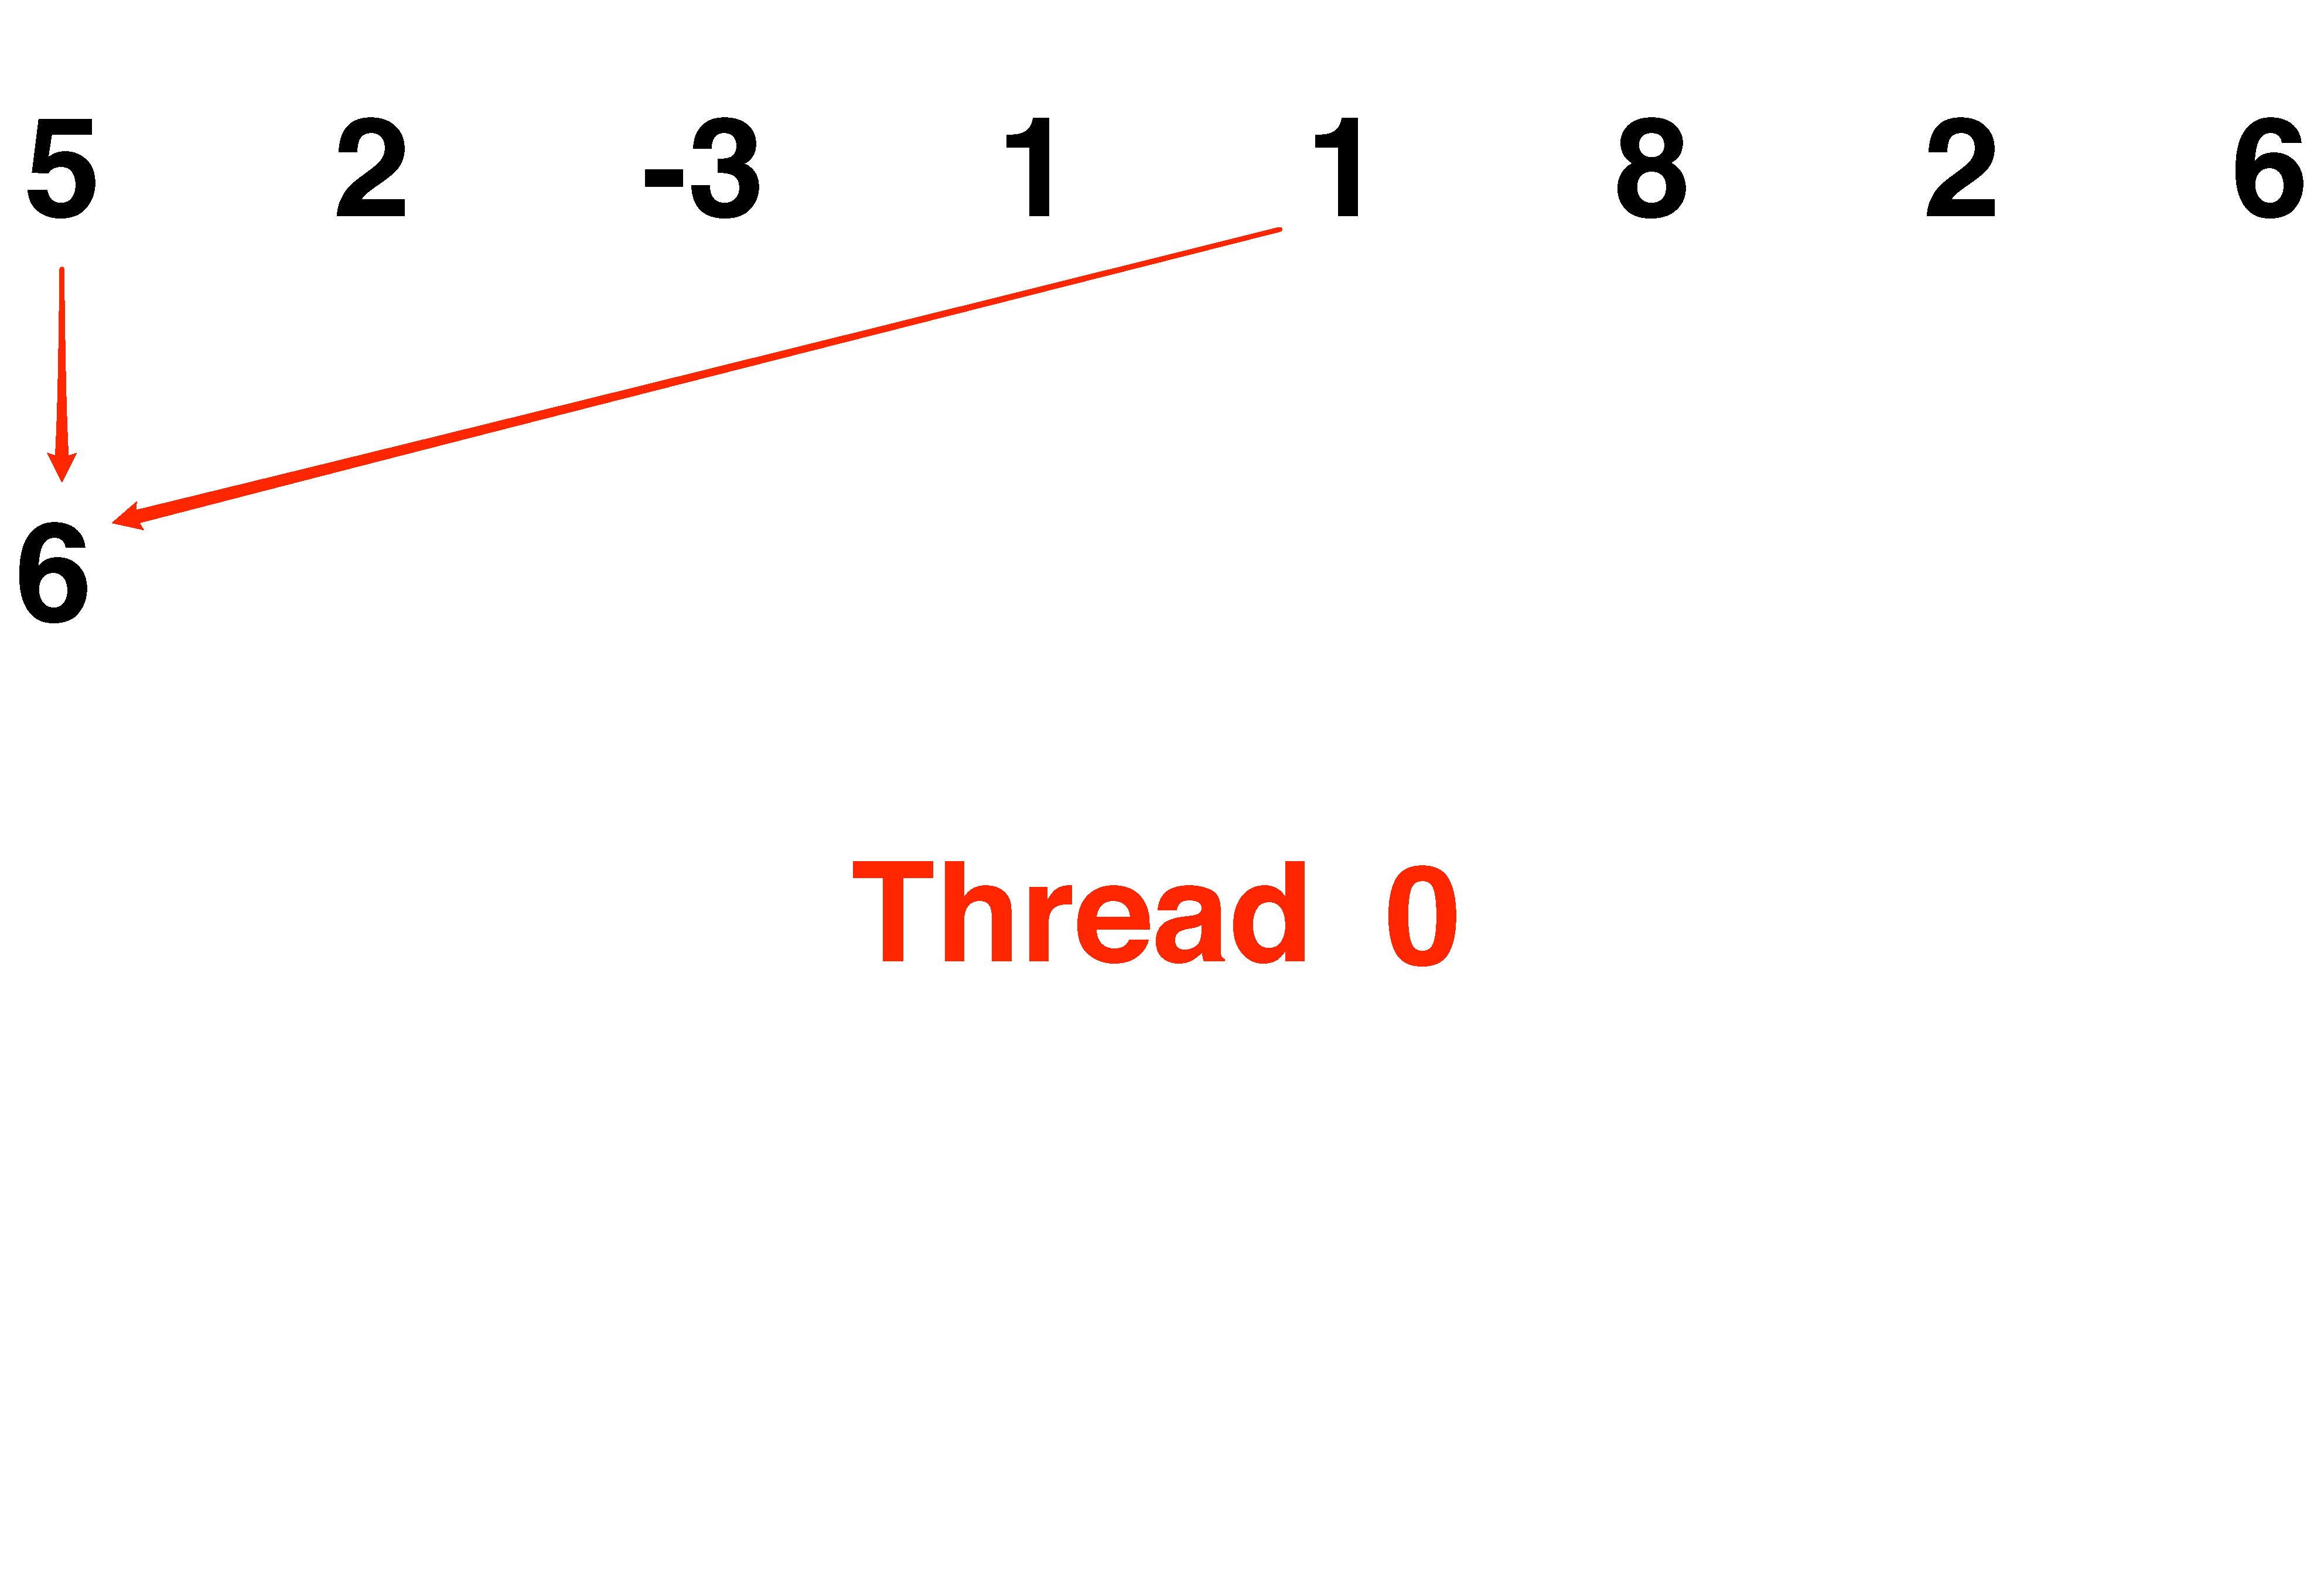
\includegraphics[scale = .15]{../../fig/psum1}
\end{center}
\end{frame}

\begin{frame}
\frametitle{Synchronizing threads within blocks: the pairwise sum revisited}
\begin{center}
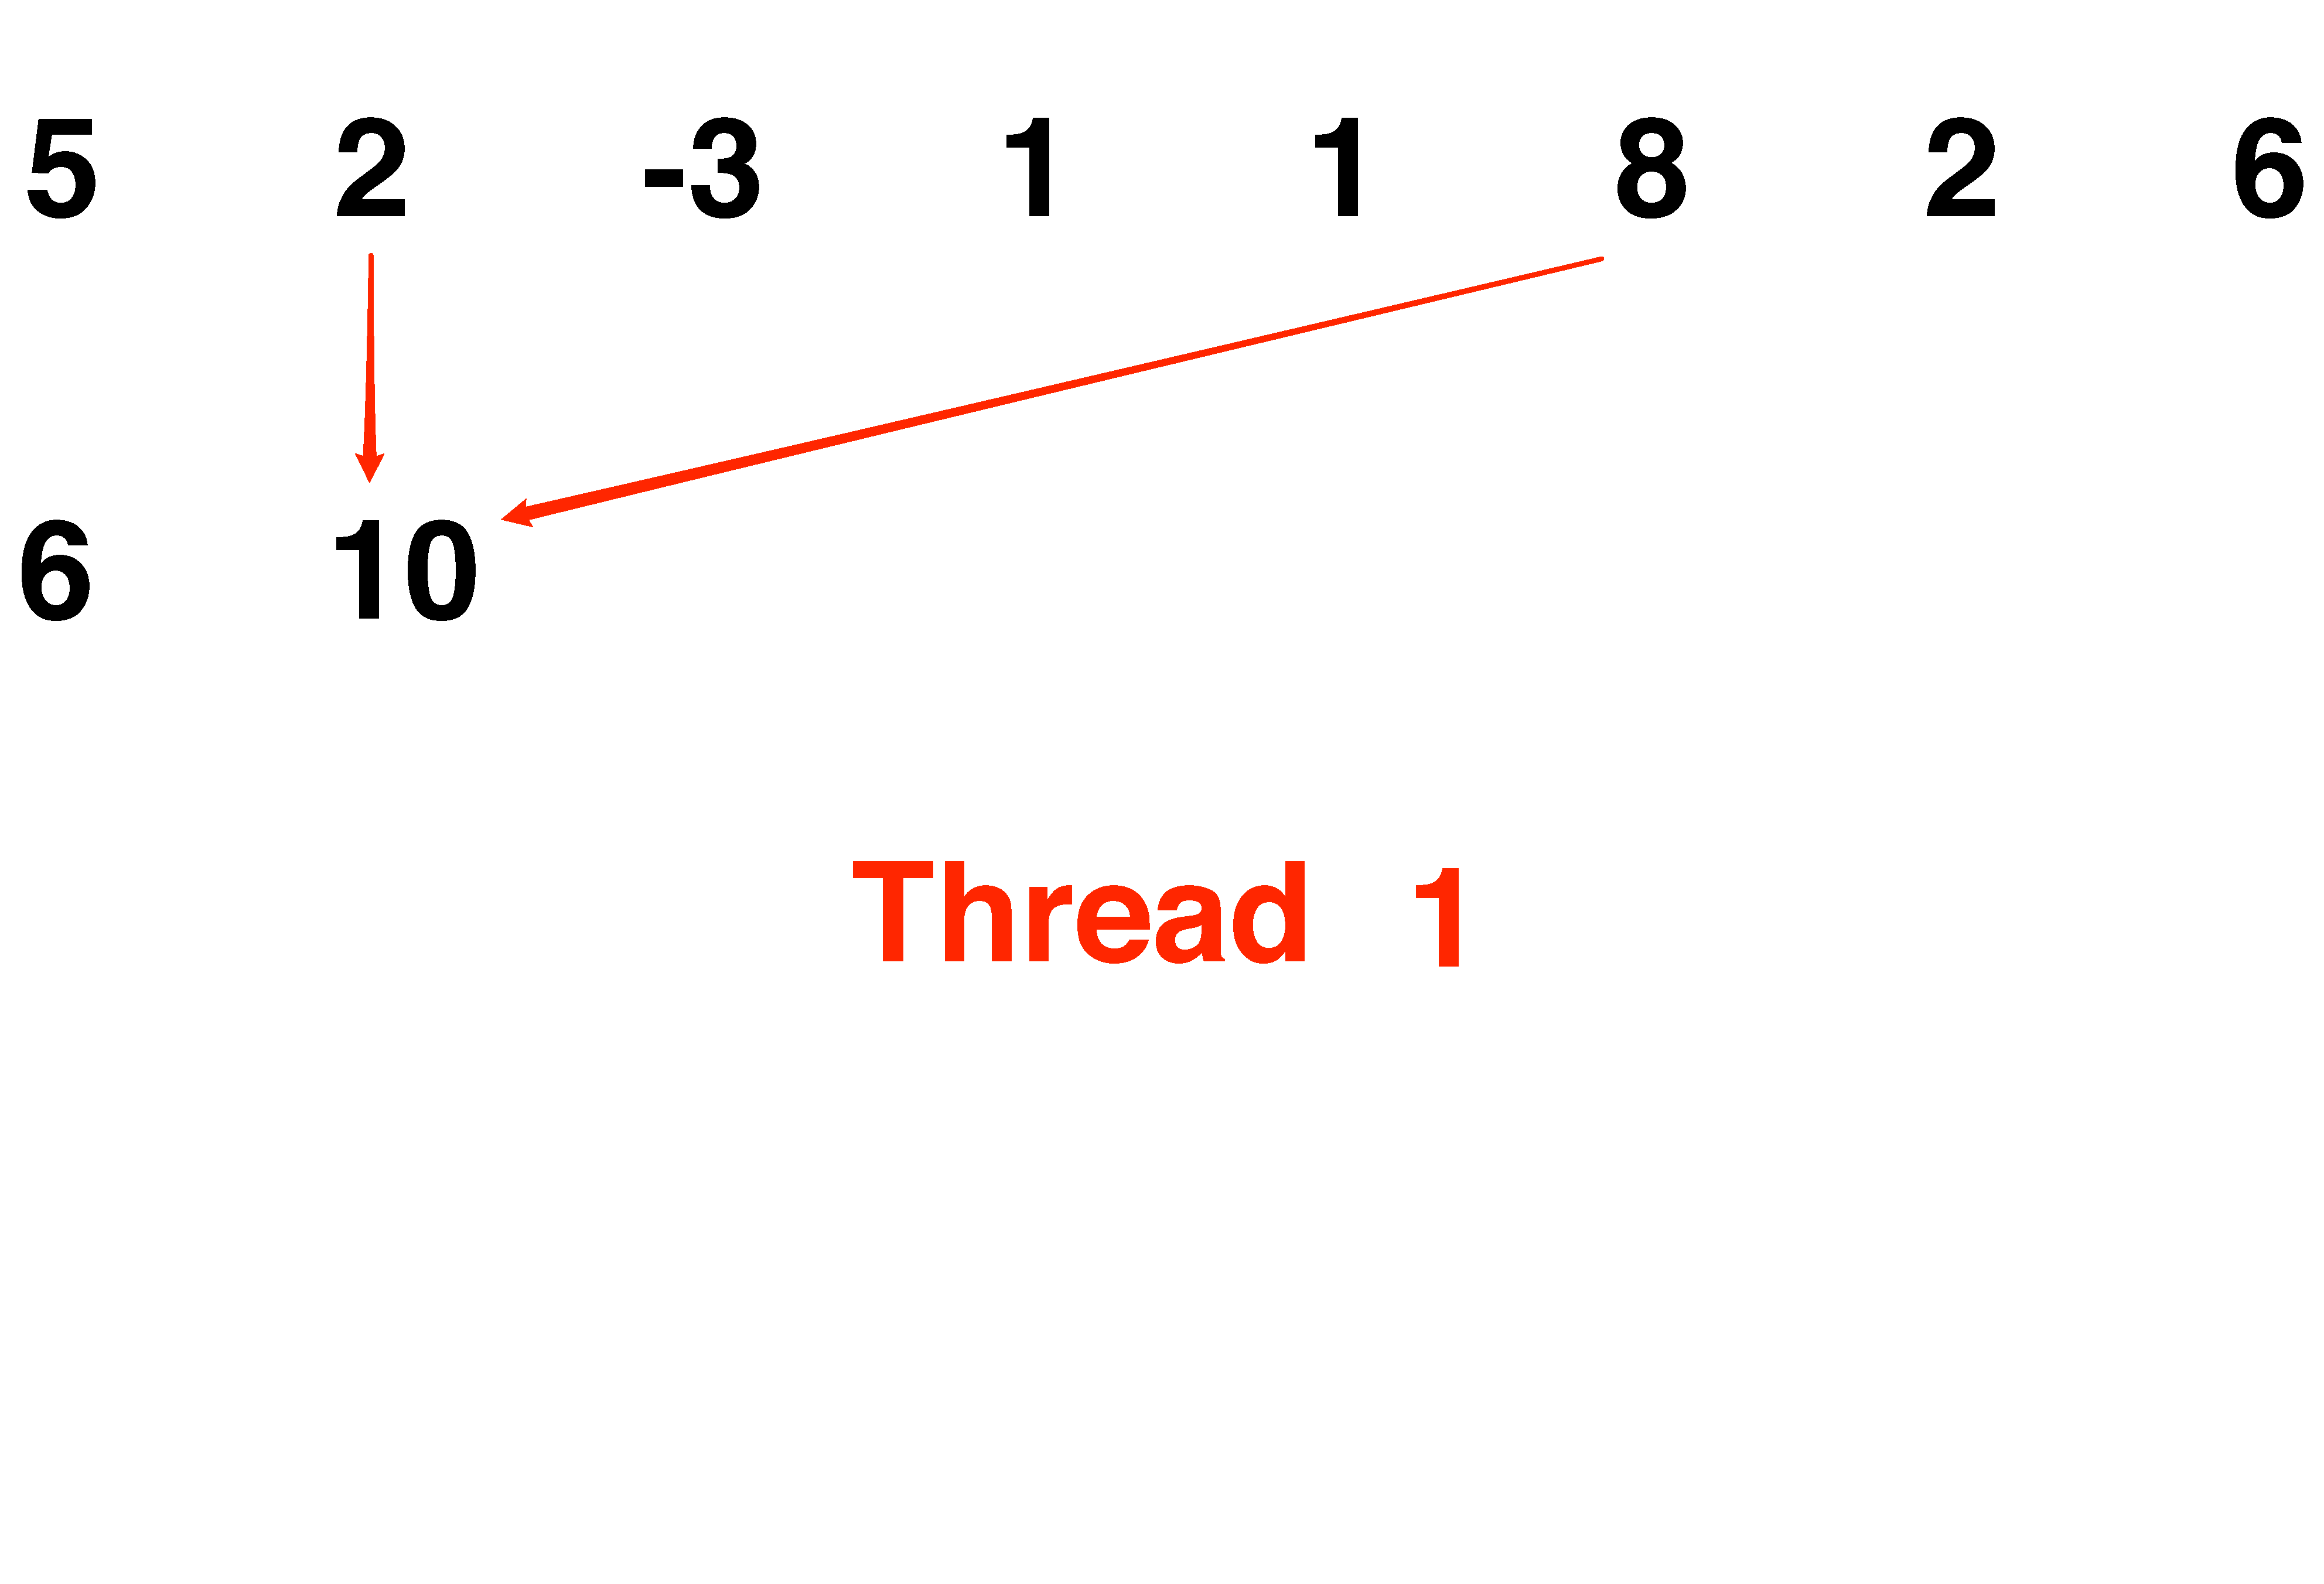
\includegraphics[scale = .15]{../../fig/psum2}
\end{center}
\end{frame}

\begin{frame}
\frametitle{Synchronizing threads within blocks: the pairwise sum revisited}
 \begin{center}
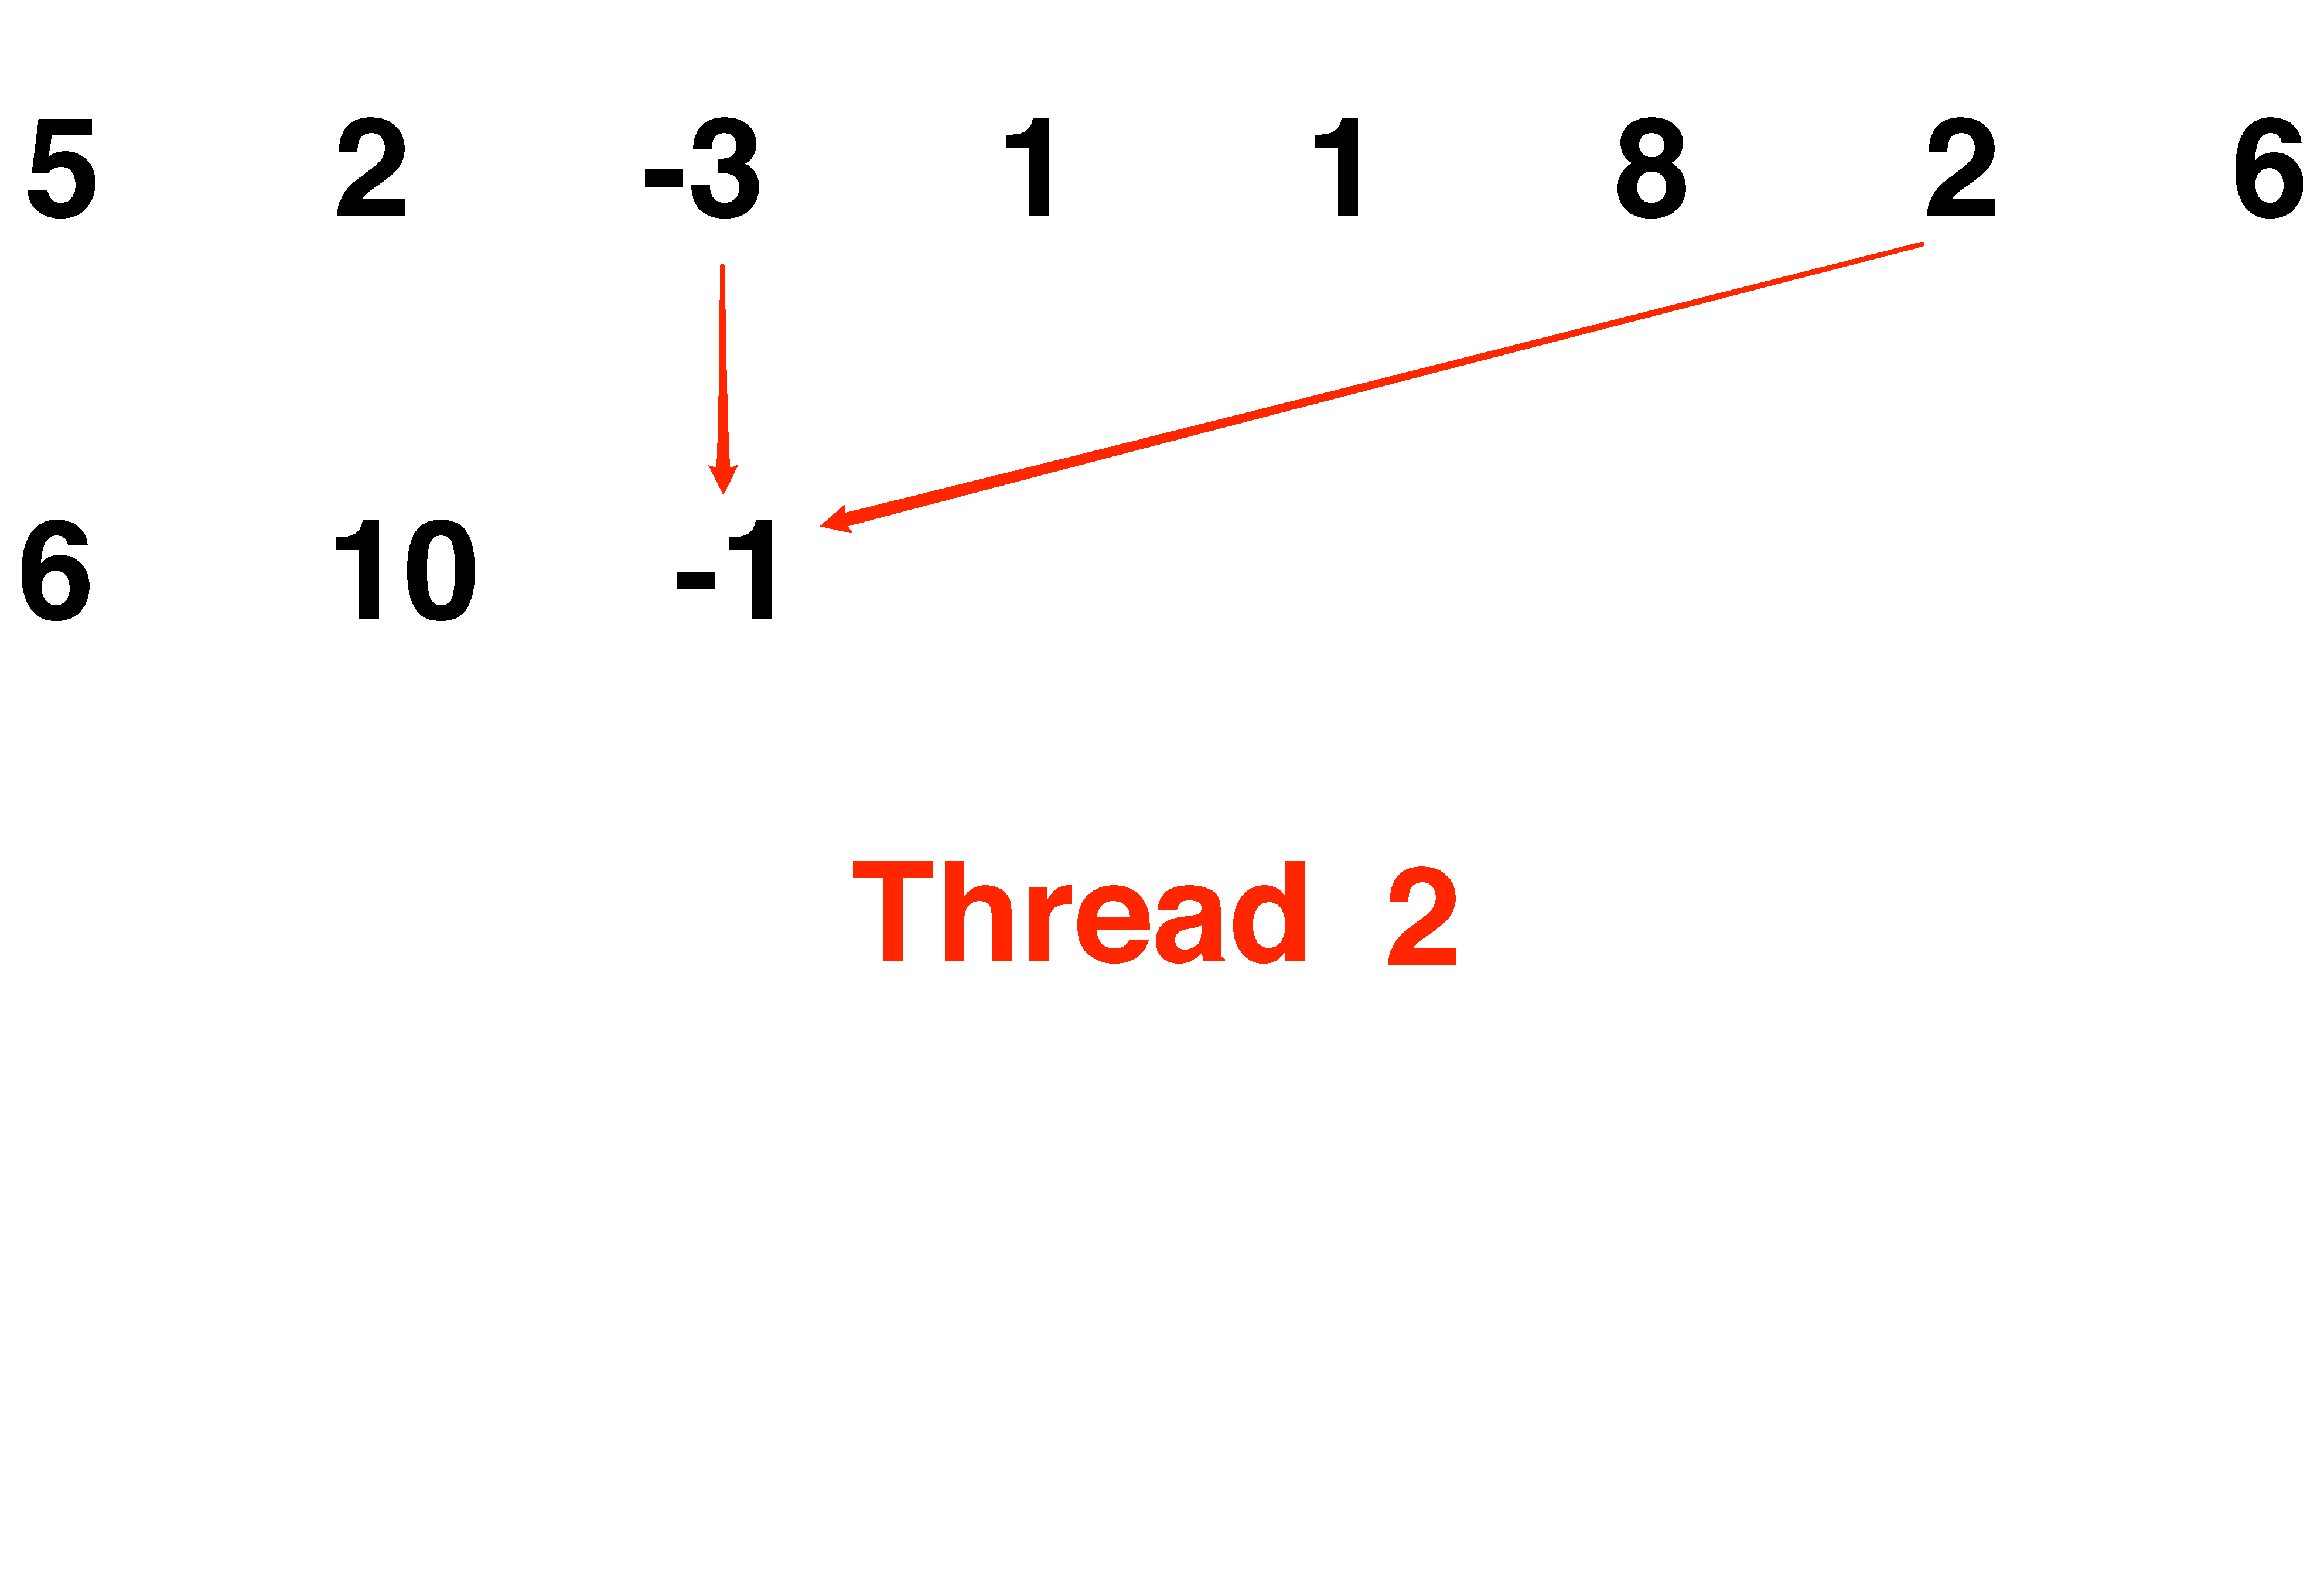
\includegraphics[scale = .15]{../../fig/psum3}
\end{center}
\end{frame}

\begin{frame}
\frametitle{Synchronizing threads within blocks: the pairwise sum revisited}
 \begin{center}
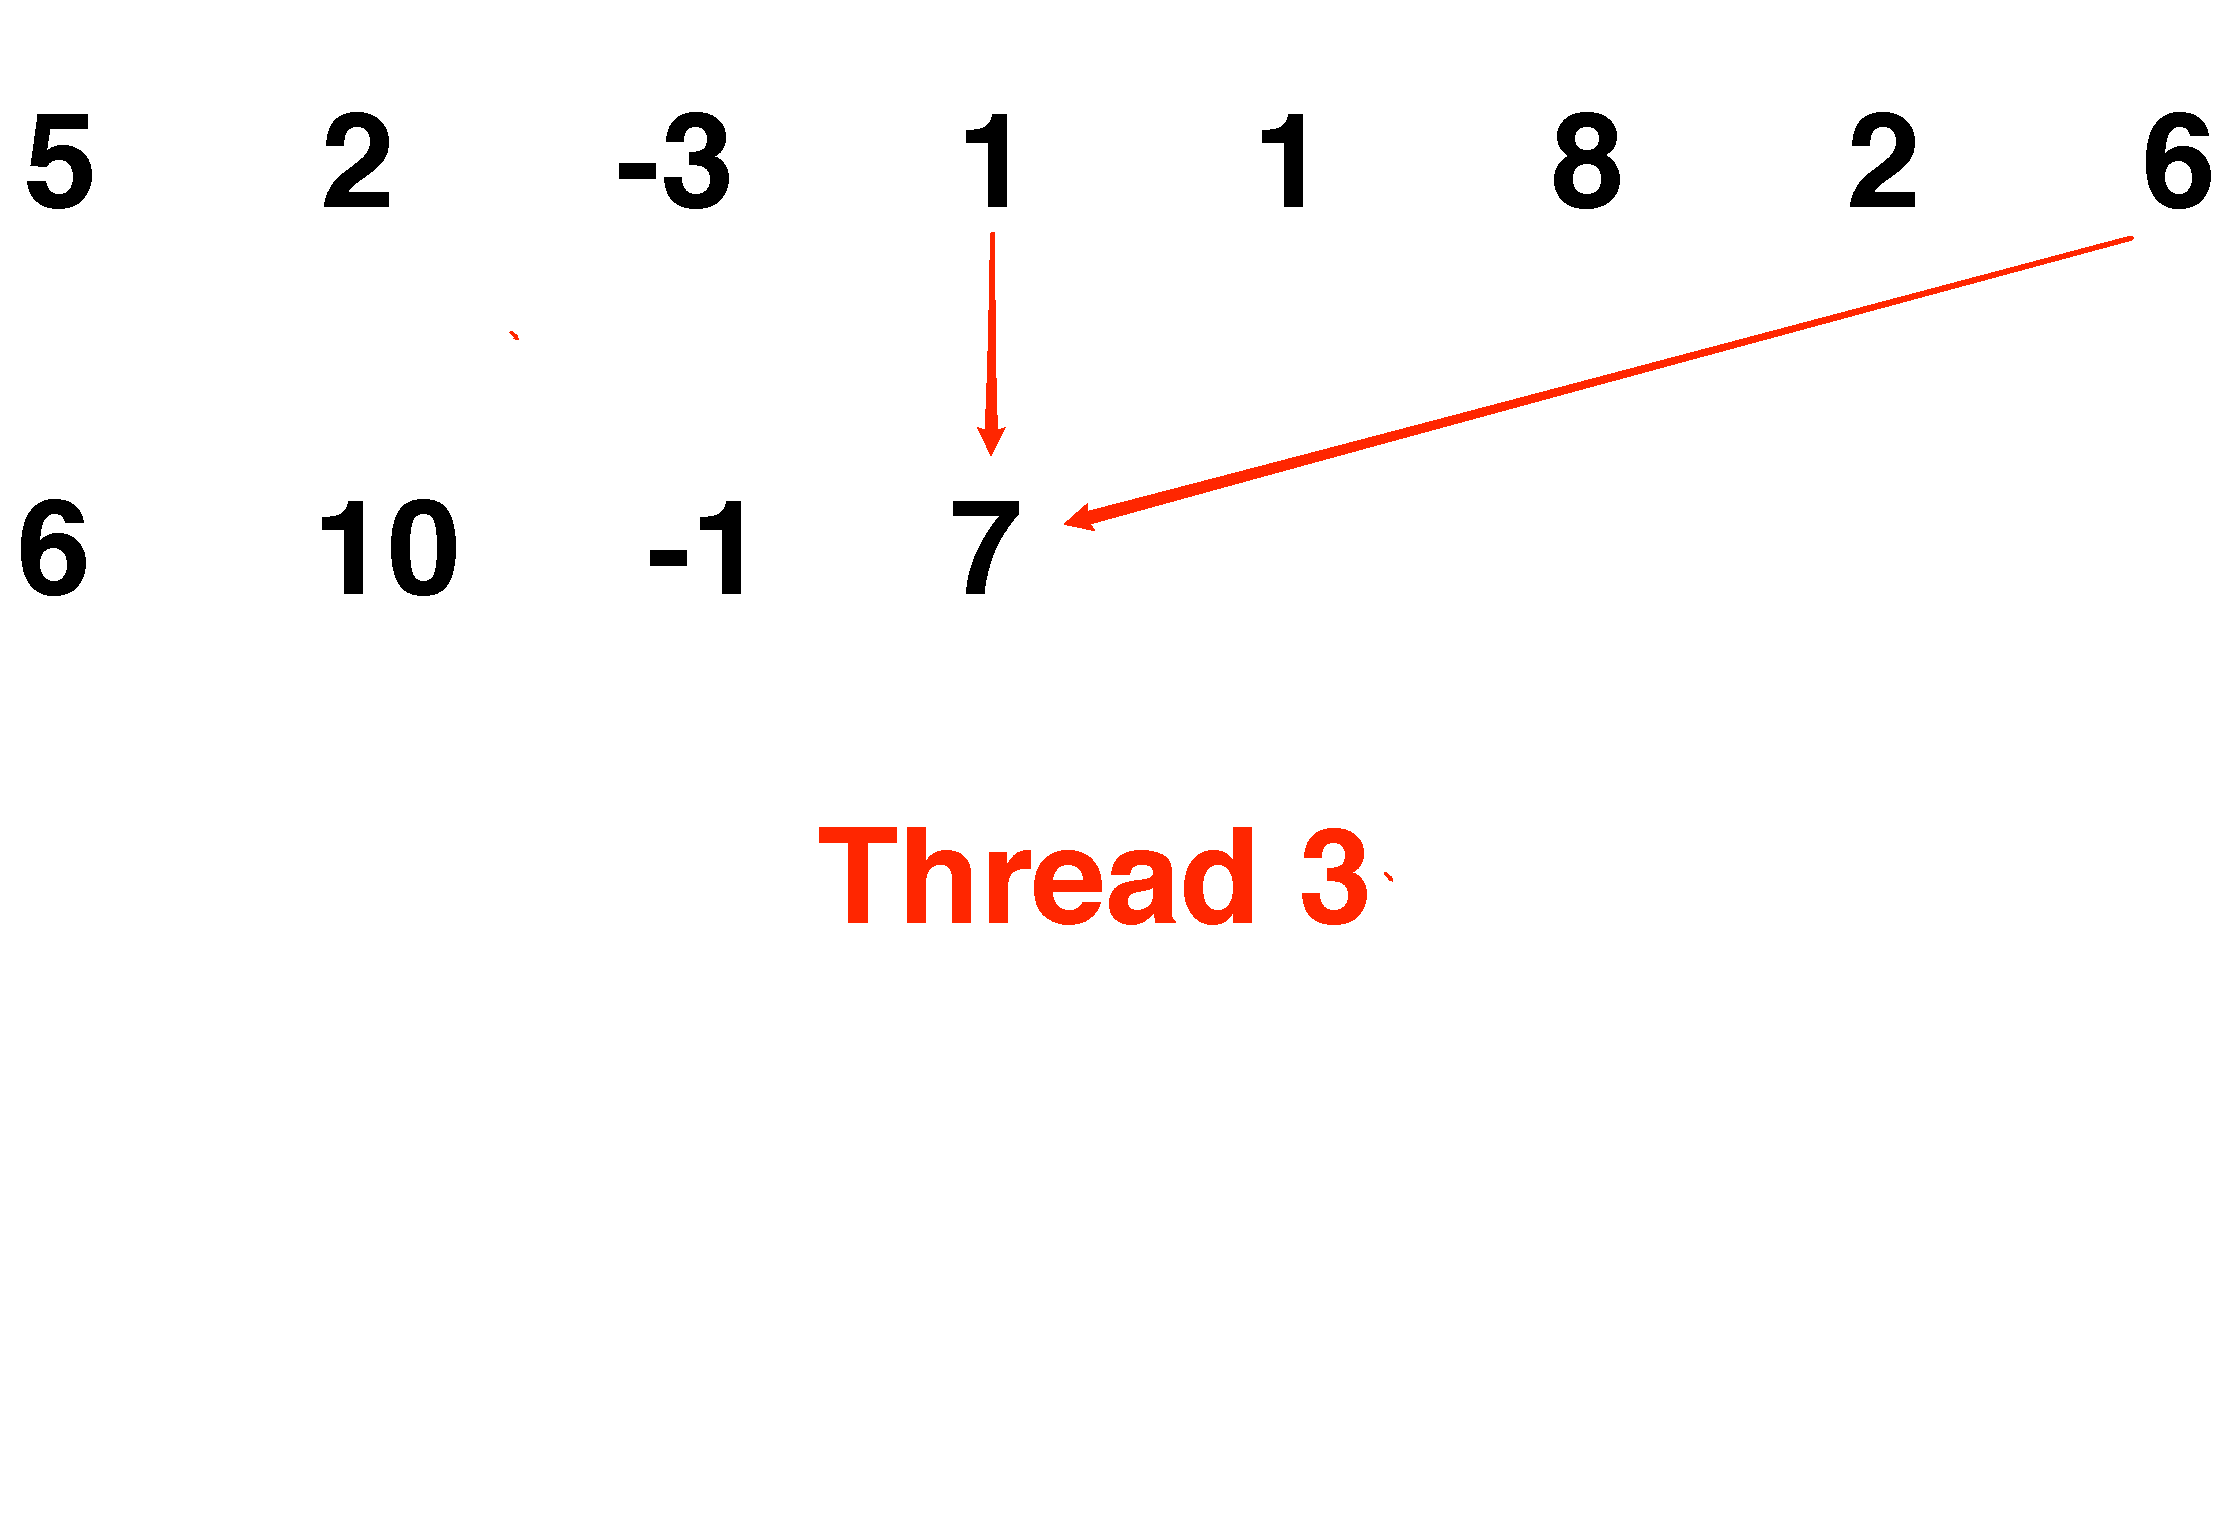
\includegraphics[scale = .25]{../../fig/psum4}
\end{center}
\end{frame}

\begin{frame}
\frametitle{Synchronizing threads within blocks: the pairwise sum revisited}
 \begin{center}
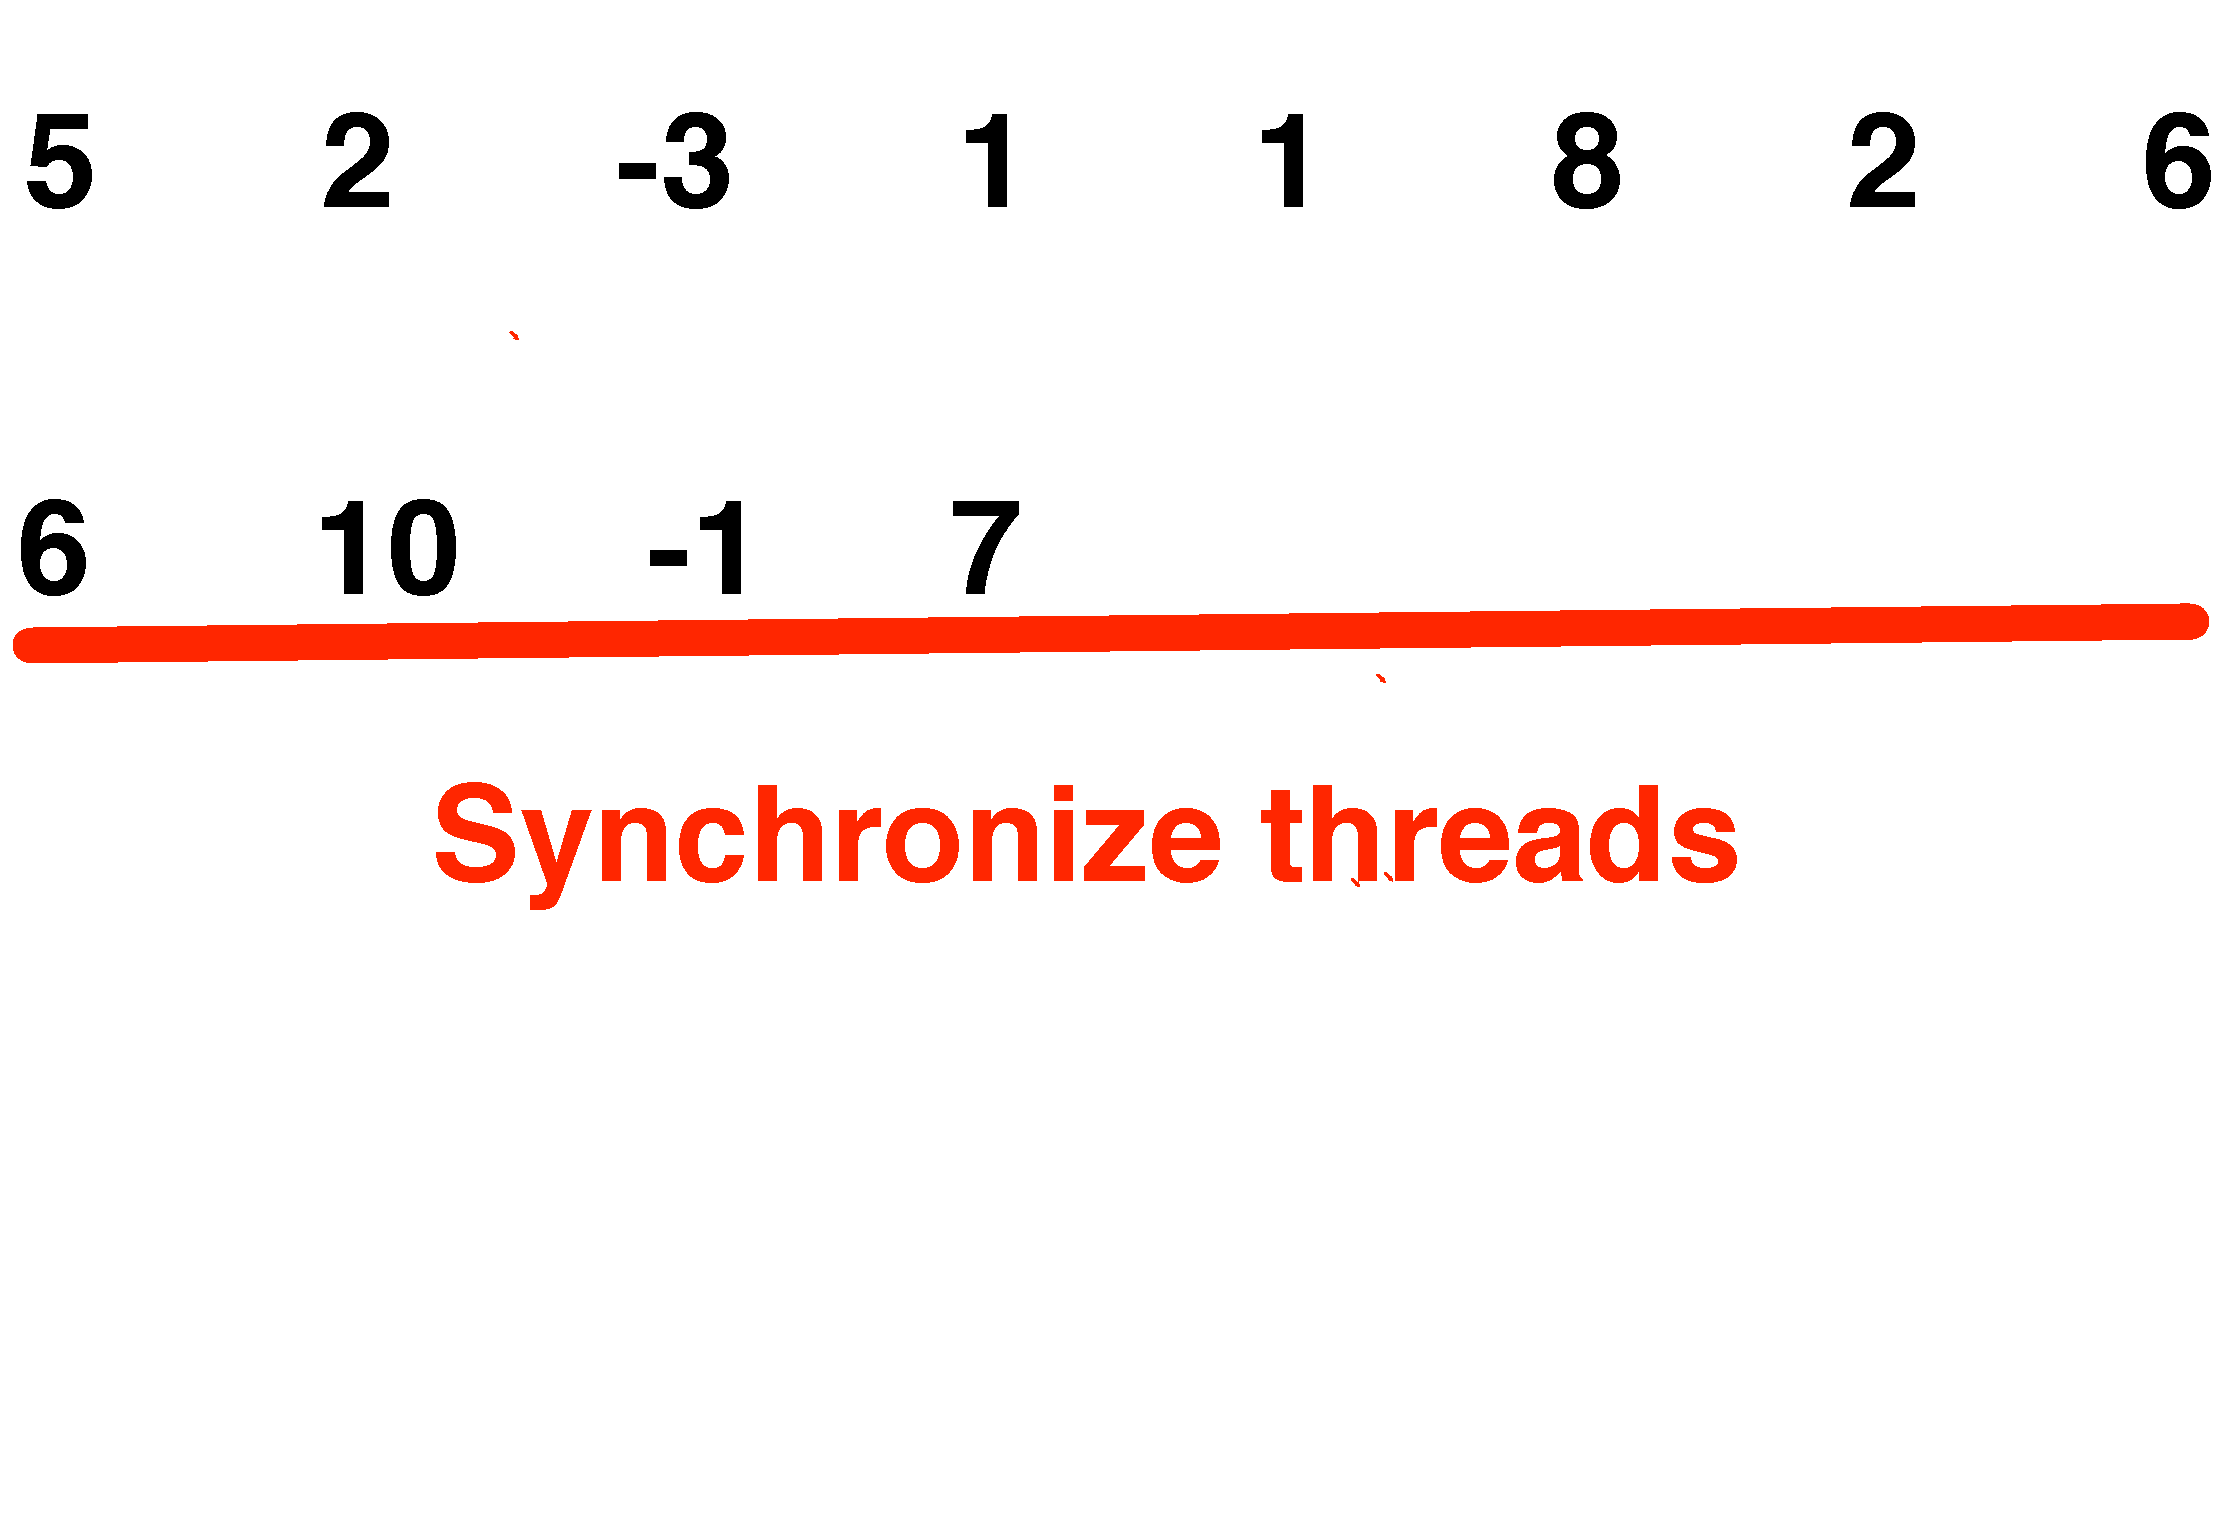
\includegraphics[scale = .25]{../../fig/psum5}
\end{center}
\end{frame}

\begin{frame}
\frametitle{Synchronizing threads within blocks: the pairwise sum revisited}
\begin{center}
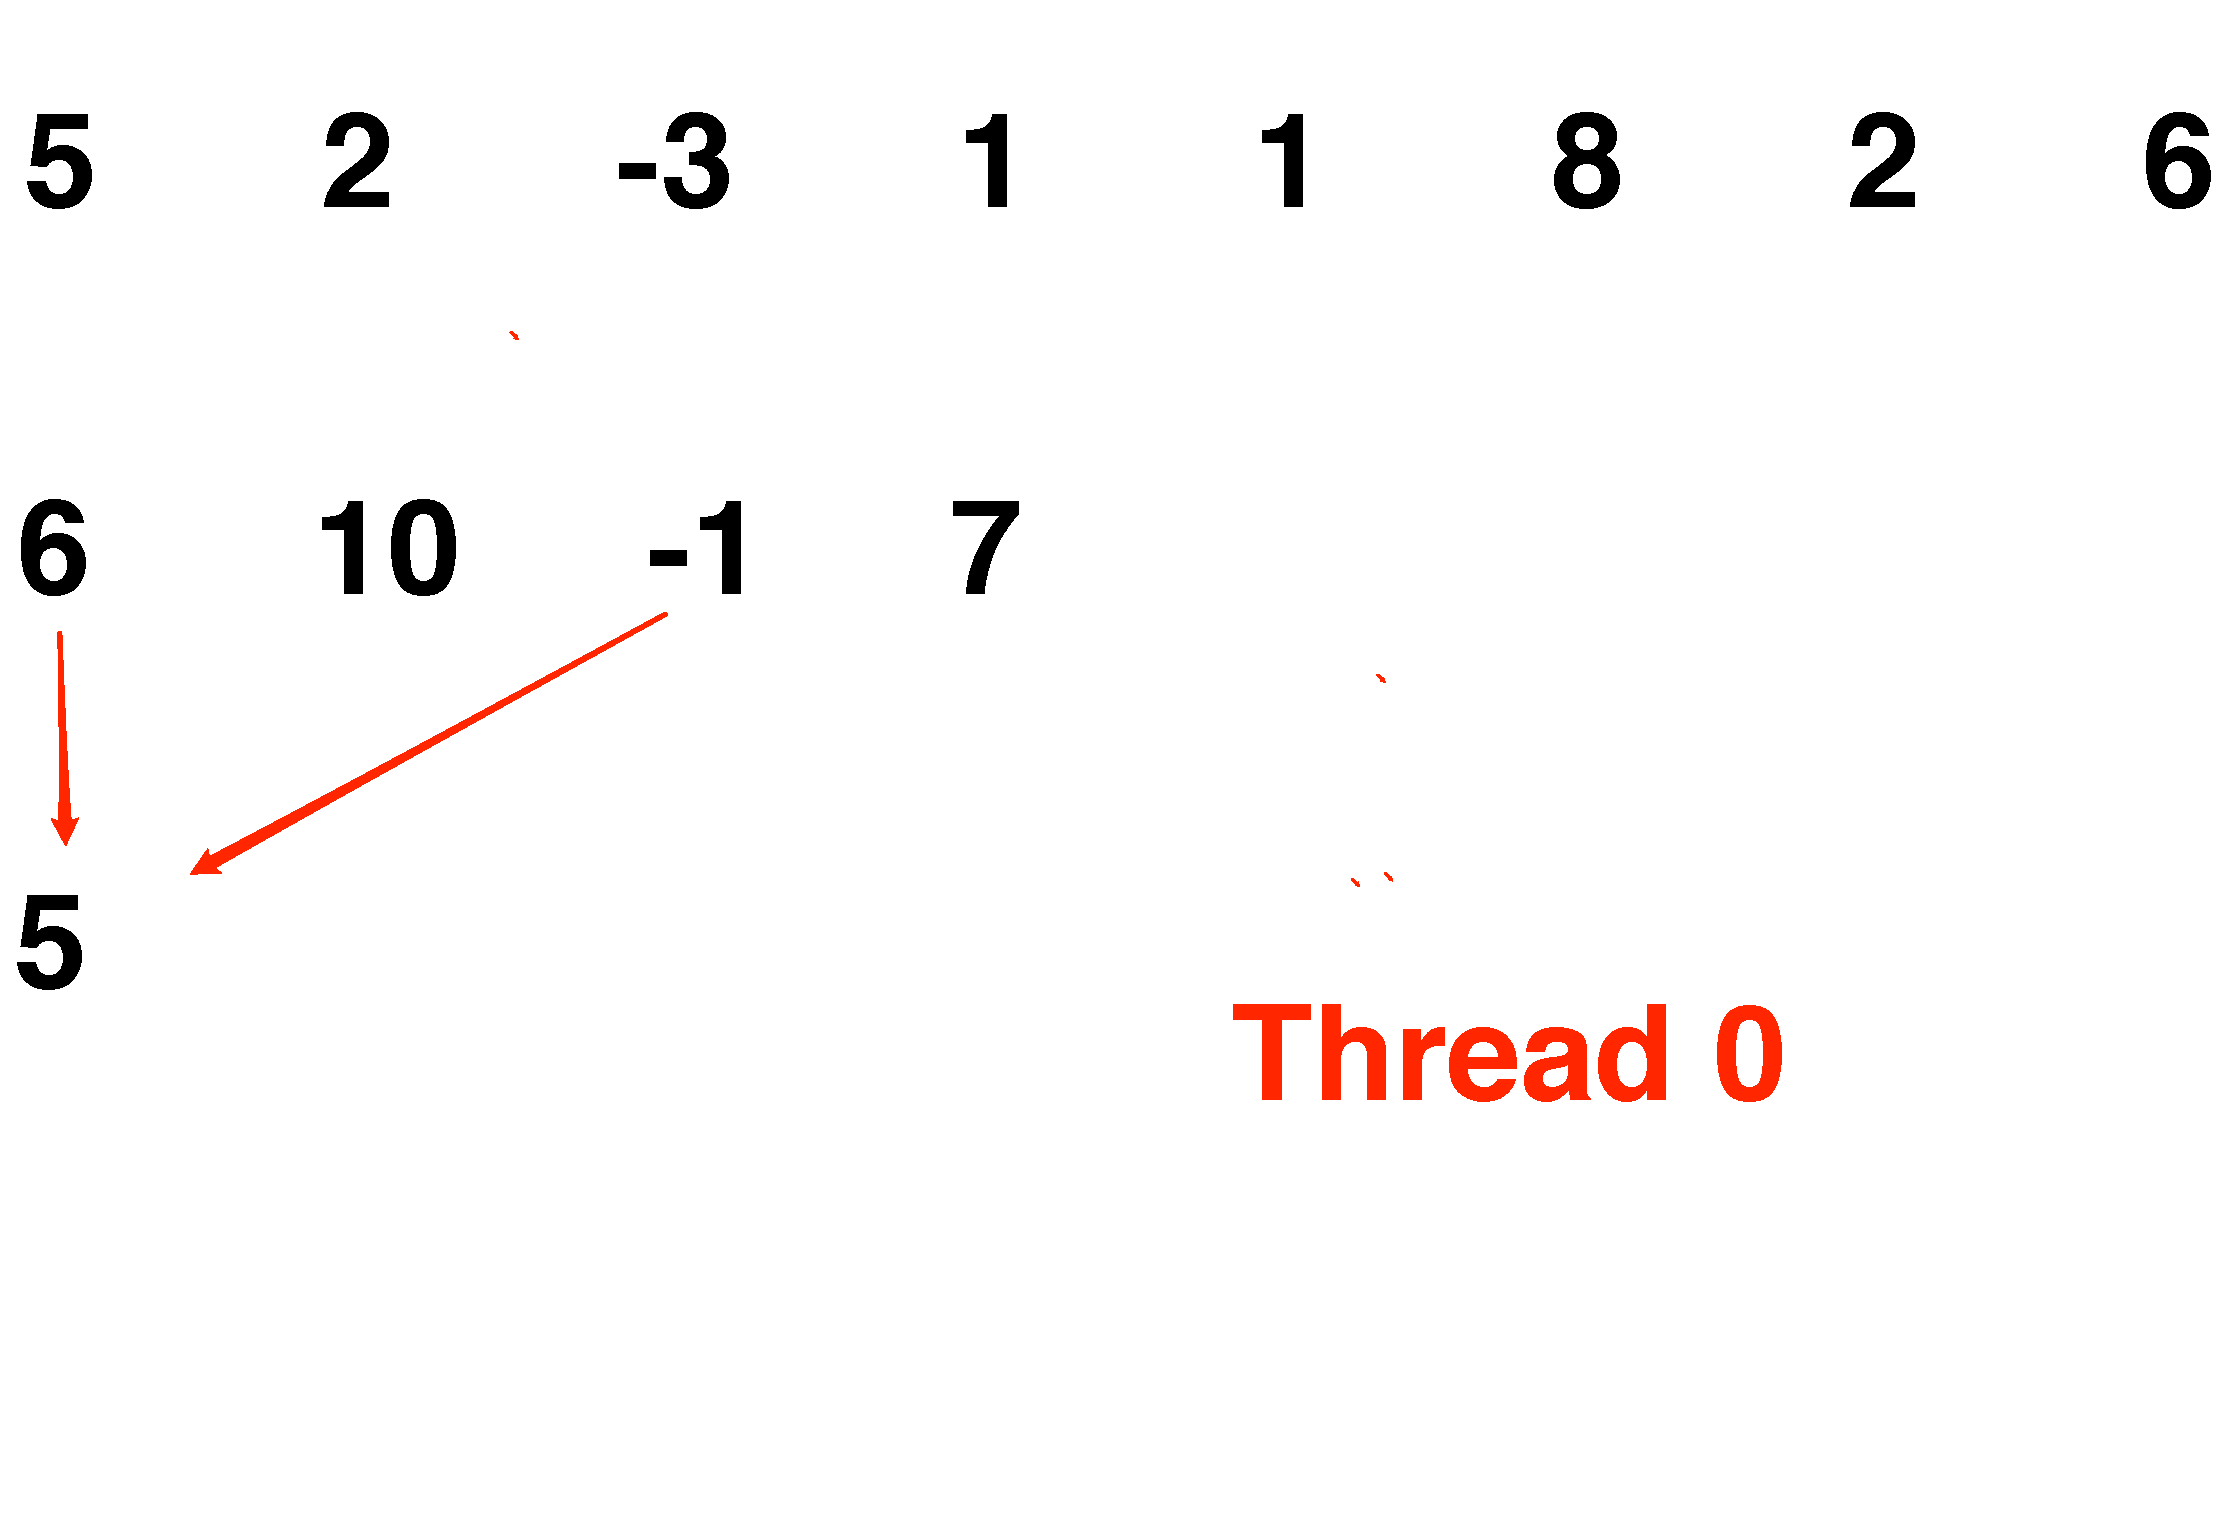
\includegraphics[scale = .25]{../../fig/psum6}
\end{center}
\end{frame}

\begin{frame}
\frametitle{Synchronizing threads within blocks: the pairwise sum revisited}
 \begin{center}
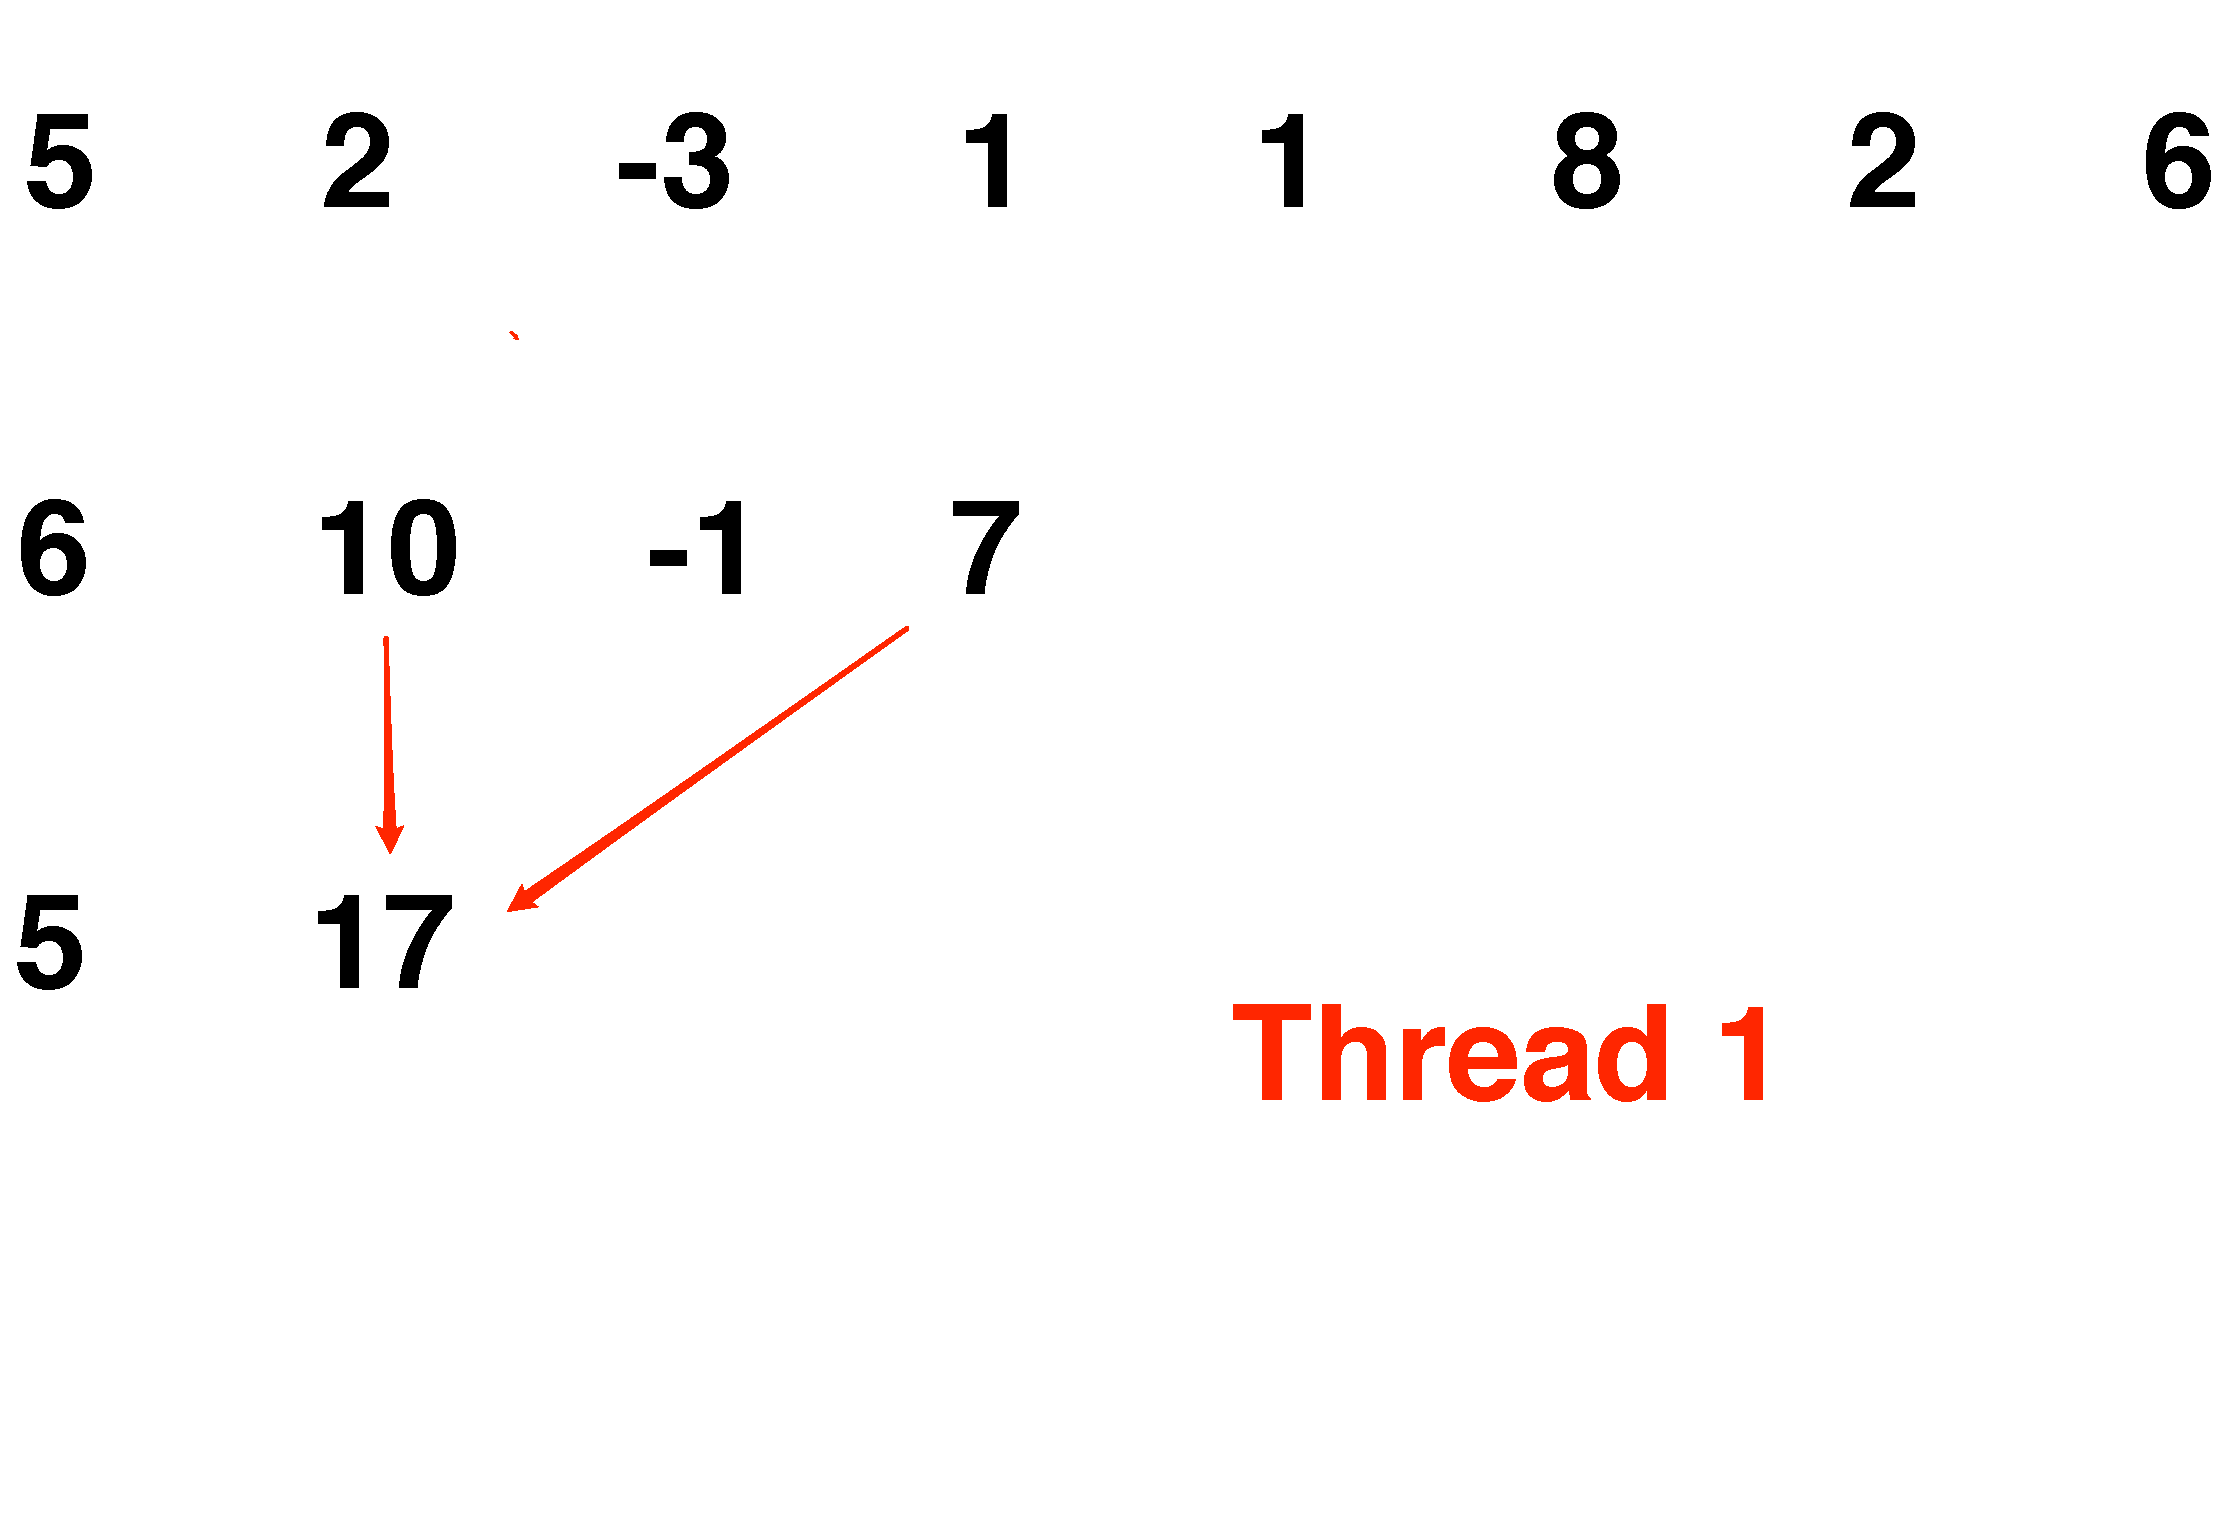
\includegraphics[scale = .25]{../../fig/psum7}
\end{center}
\end{frame}

\begin{frame}
\frametitle{Synchronizing threads within blocks: the pairwise sum revisited}
 \begin{center}
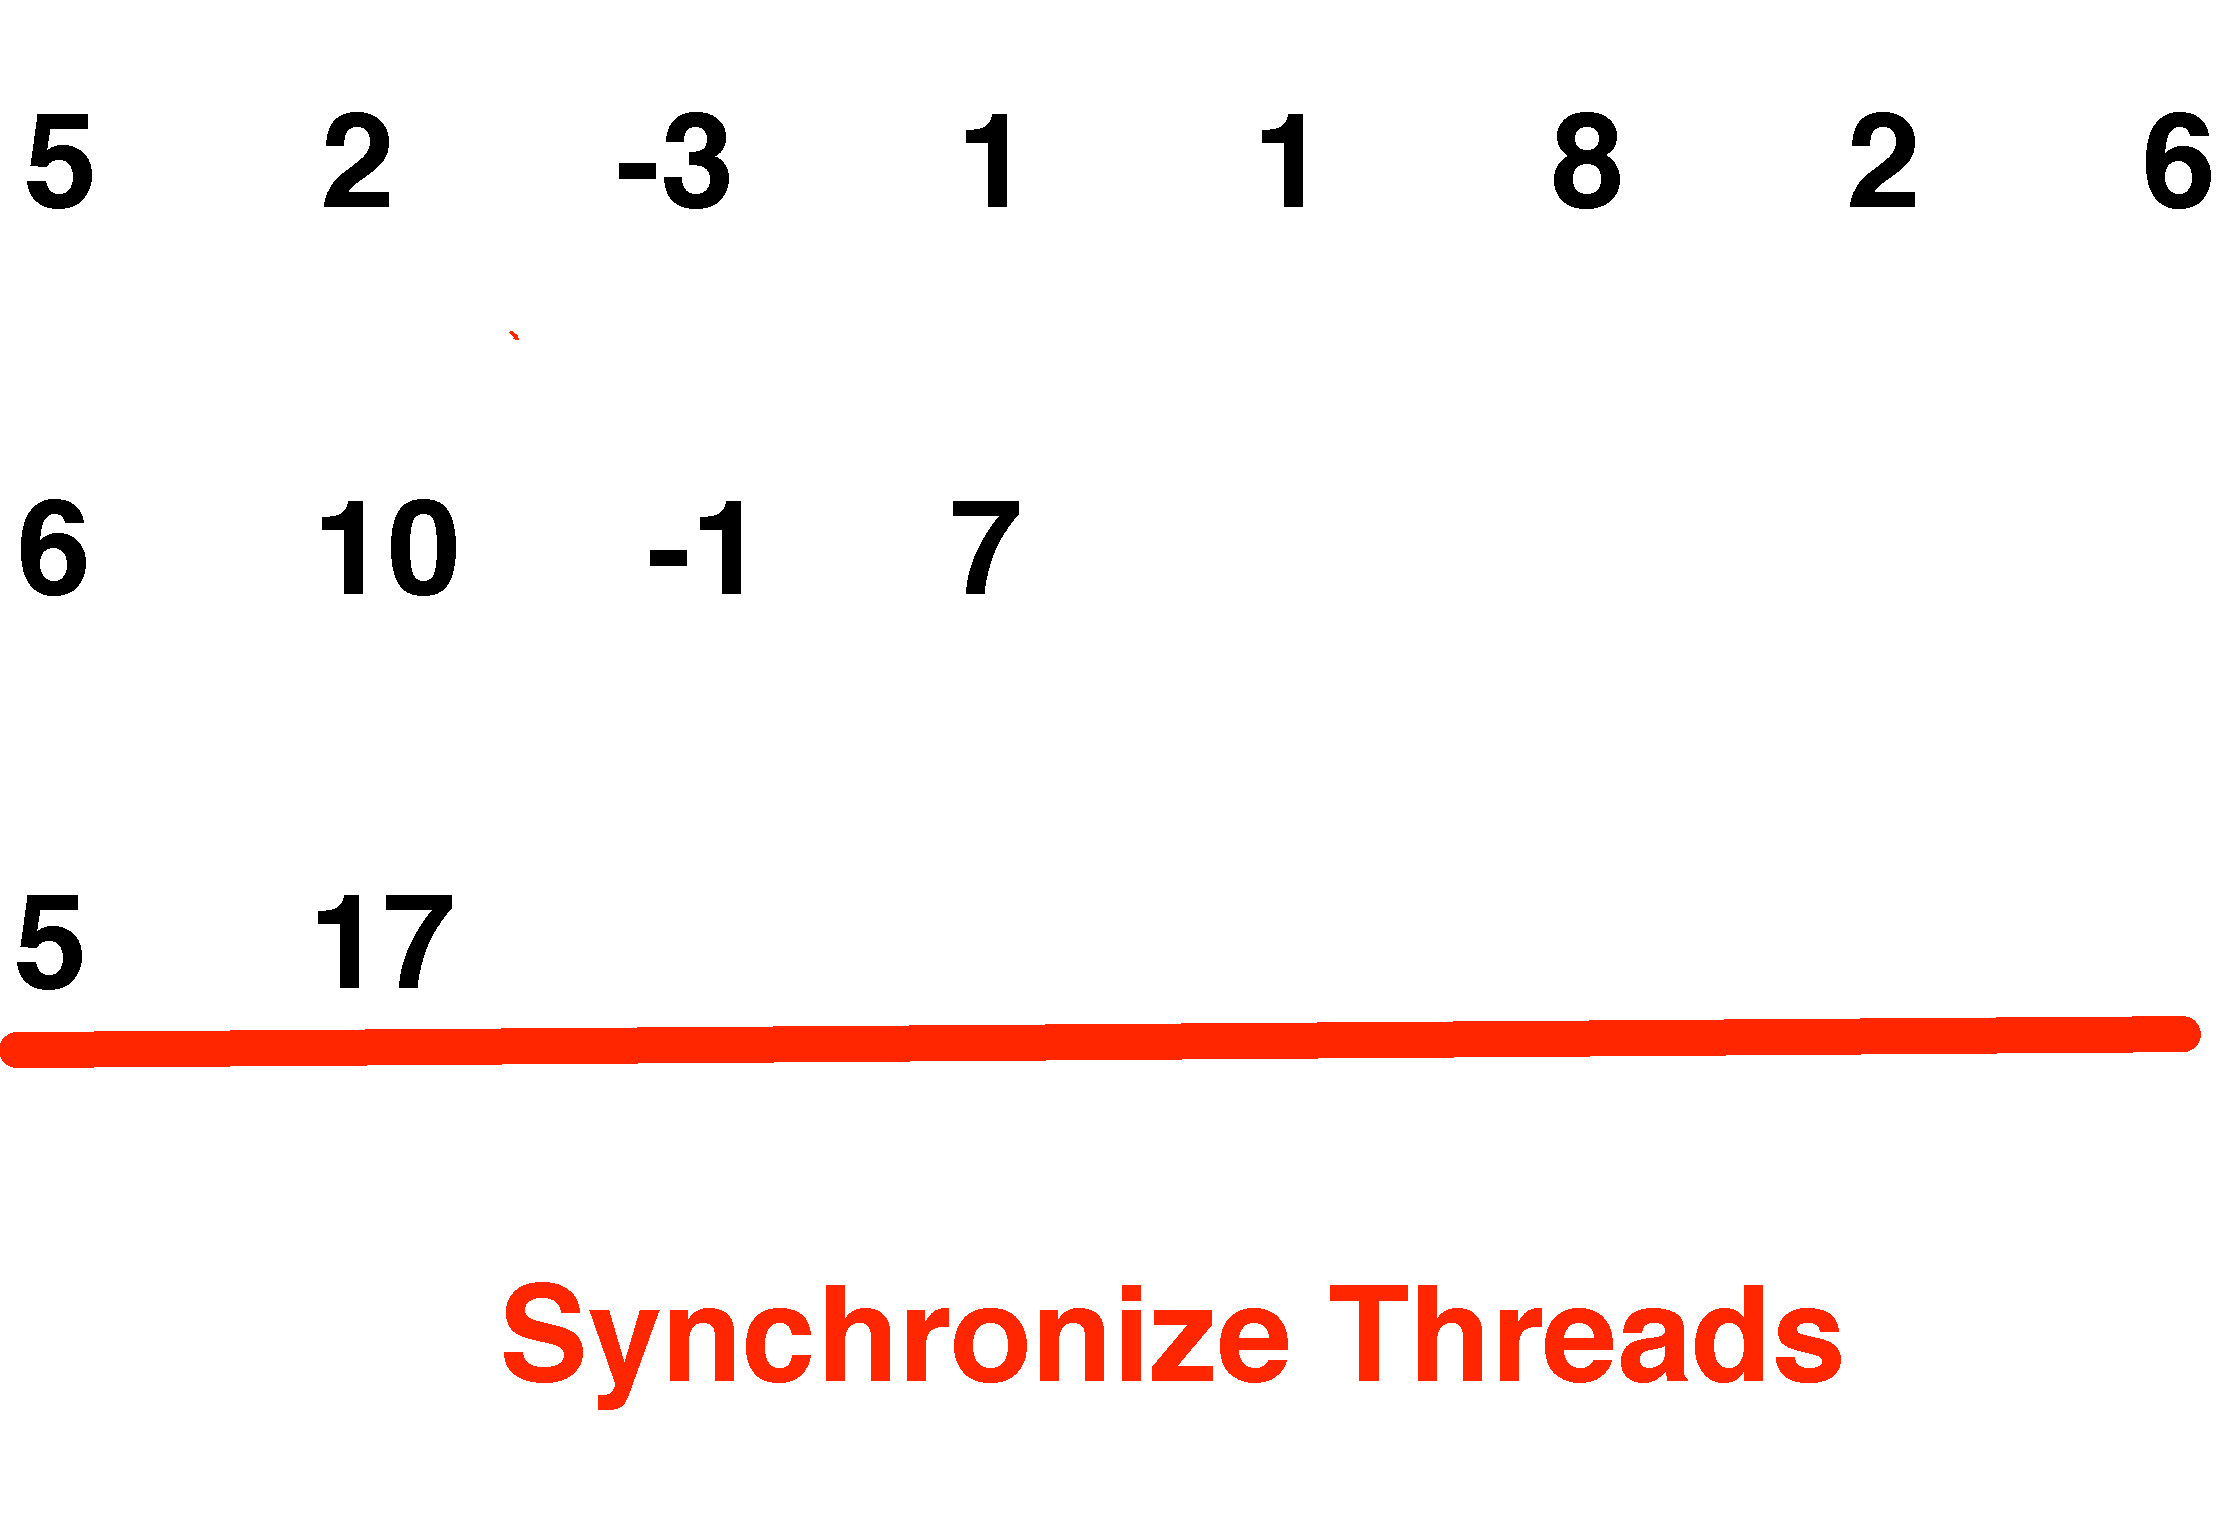
\includegraphics[scale = .25]{../../fig/psum8}
\end{center}
\end{frame}

\begin{frame}
\frametitle{Synchronizing threads within blocks: the pairwise sum revisited} \begin{center}
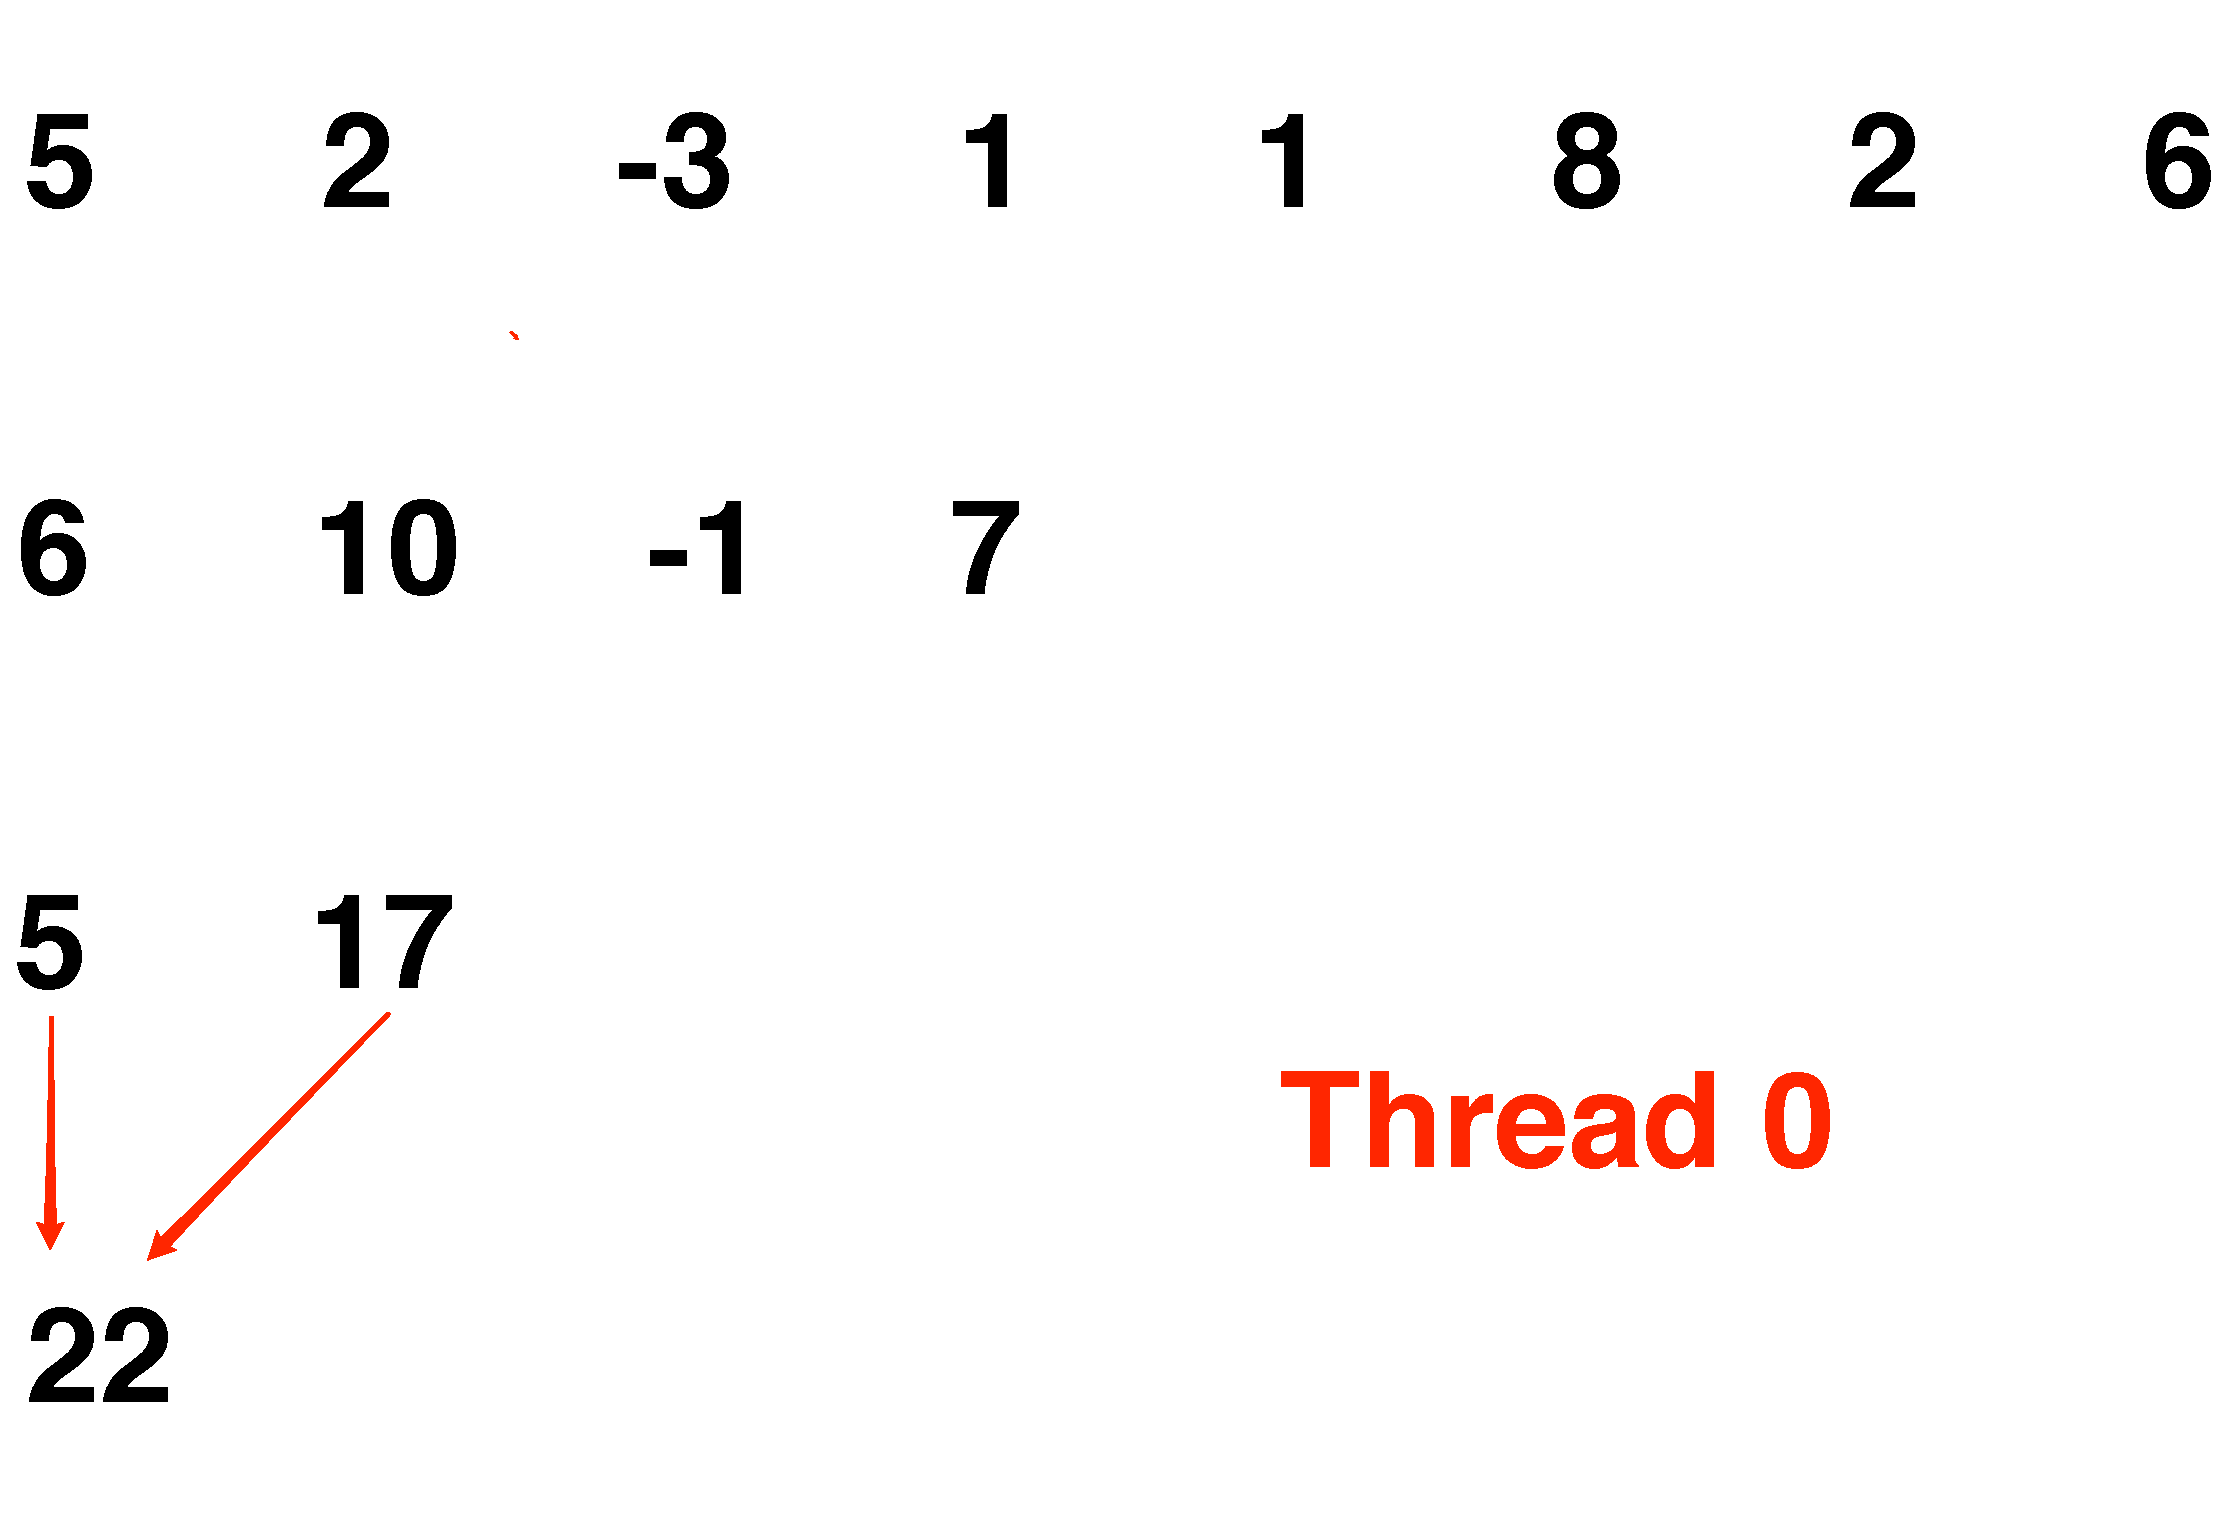
\includegraphics[scale = .25]{../../fig/psum9}
\end{center}
\end{frame}

\begin{frame}[fragile]
\frametitle{Pairwise sum in pseudocode}
\begin{itemize}
\item Let $n = 2^m$ be the length of the vector.
\pause \item Denote the vector by $(x_{(0, \ 0)}, \ldots, x_{(0, \ n - 1)})$
\pause \item Spawn 1 grid with a single block of $n/2$ threads. 
\pause \item Do:
\begin{enumerate}
 \item Set offset = $n / 2$.
\pause \item For parallel threads $j= 0, \ldots, \text{offset} - 1$, compute:
\begin{align*}
x_{(i, \ j)} = x_{(i-1, \ j)} + x_{(i - 1, \ j + \text{offset})}
\end{align*}
\pause \item Synchronize threads.
\pause \item Integer divide offset by 2.
\pause \item Return to step 2 if $\text{offset} > 0$.
\end{enumerate}
\end{itemize}
\end{frame}



\begin{frame}[fragile]
\frametitle{{\tt pairwise\_sum.cu}}\lstset{basicstyle=\tiny}
\begin{lstlisting}[name=psum]
#include <stdio.h> 
#include <stdlib.h> 
#include <math.h>
#include <cuda.h>
#include <cuda_runtime.h> 

/*
 * This program computes the sum of the elements of 
 * vector v using the pairwise (cascading) sum algorithm.
 */

#define N 8 // length of vector v. MUST BE A POWER OF 2!!!

// Fill the vector v with n random floating point numbers.
void vfill(float* v, int n){
  int i;
  for(i = 0; i < n; i++){
    v[i] = (float) rand() / RAND_MAX;
  }
}

// Print the vector v.
void vprint(float* v, int n){
  int i;
  printf("v = \n");
  for(i = 0; i < n; i++){
    printf("%7.3f\n", v[i]);
  }
  printf("\n");
}
\end{lstlisting}
\end{frame}


\begin{frame}[fragile]
\frametitle{{\tt pairwise\_sum.cu}} \lstset{basicstyle=\tiny}
\begin{lstlisting}[name=psum]
// Pairwise-sum the elements of vector v and store the result in v[0]. 
__global__ void psum(float* v){ 
  int t = threadIdx.x; // Thread index.
  int n = blockDim.x; // Should be half the length of v.

  while (n != 0) {
    if(t < n)
      v[t] += v[t + n];  
    __syncthreads();    
    n /= 2; 
  }
}

int main (void){ 
  float *v_h, *v_d; // host and device copies of our vector, respectively
  
  // dynamically allocate memory on the host for v_h
  v_h = (float*) malloc(N * sizeof(*v_h)); 
  
  // dynamically allocate memory on the device for v_d
  cudaMalloc ((float**) &v_d, N *sizeof(*v_d)); 
  
  // Fill v_h with N random floating point numbers.
  vfill(v_h, N);
  
  // Print v_h to the console
  vprint(v_h, N);
\end{lstlisting}
\end{frame}


\begin{frame}[fragile]
\frametitle{{\tt pairwise\_sum.cu}} \lstset{basicstyle=\tiny}
\begin{lstlisting}[name=psum]
  // Write the contents of v_h to v_d
  cudaMemcpy( v_d, v_h, N * sizeof(float), cudaMemcpyHostToDevice );
  
  // Compute the pairwise sum of the elements of v_d and store the result in v_d[0].
  psum<<< 1, N/2 >>>(v_d);
  
  // Write the pairwise sum, v_d[0], to v_h[0].
  cudaMemcpy(v_h, v_d, sizeof(float), cudaMemcpyDeviceToHost );

  // Print the pairwise sum.
  printf("Pairwise sum = %7.3f\n", v_h[0]);
  
  // Free dynamically-allocated host memory
  free(v_h);

  // Free dynamically-allocated device memory    
  cudaFree(v_d);
}
\end{lstlisting}
\end{frame}

\begin{frame}[fragile]
\frametitle{Compiling and running {\tt pairwise\_sum.cu}}
\begin{lstlisting}
> nvcc pairwise_sum.cu -o pairwise_sum
> ./pairwise_sum
v =
  0.840
  0.394
  0.783
  0.798
  0.912
  0.198
  0.335
  0.768
  
Pairwise sum =   5.029
\end{lstlisting}
\end{frame}


\subsection{Respecting the SIMD paradigm}

\begin{frame}
\frametitle{Best practices: respect the SIMD paradigm}
\begin{itemize}
\pause \item SIMD: ``Single Instruction, Multiple Data"
\pause \item Under this paradigm, the thread in a kernel call write to different memory spaces.
\pause \item When threads write to the same memory (SISD), problems can arise.
\end{itemize}
\end{frame}

\begin{frame}[fragile]
\frametitle{{\tt sisd.cu}: violating the SIMD paradigm} \lstset{basicstyle=\tiny}
\begin{lstlisting}
#include <stdio.h>
#include <stdlib.h>
#include <cuda.h>
#include <cuda_runtime.h> 

__global__ void colonel(int *a_d){
  *a_d = blockDim.x * blockIdx.x + threadIdx.x;
}

int main(){

  int a = 0, *a_d;
  
  cudaMalloc((void**) &a_d, sizeof(int));
  cudaMemcpy(a_d, &a, sizeof(int), cudaMemcpyHostToDevice);

  colonel<<<4,5>>>(a_d); 
  
  cudaMemcpy(&a, a_d, sizeof(int), cudaMemcpyDeviceToHost);

  printf("a = %d\n", a);
  cudaFree(a_d);

}
\end{lstlisting}

\begin{itemize}
\pause \item What is the output?
\end{itemize}
\end{frame}

\begin{frame}[fragile]
\frametitle{{\tt sisd.cu}: violating the SIMD paradigm}
\begin{lstlisting}
> nvcc sisd.cu -o sisd
> ./sisd
a = 14
\end{lstlisting}

\begin{itemize}
\pause \item The output is unpredictable because the threads modify the same variable in an unpredictable order.
\end{itemize}
\end{frame}

\begin{frame}
\frametitle{Outline}
\tableofcontents
\end{frame}

\begin{frame}
\frametitle{Resources} \small

\begin{itemize}
\item Texts:
\begin{enumerate}
 \item J. Sanders and E. Kandrot. {CUDA by Example.} Addison-Wesley, 2010.
\pause \item D. Kirk, W.H. Wen-mei, and W. Hwu. \emph{Programming massively parallel processors: a hands-on approach.} Morgan Kaufmann, 2010.
\end{enumerate}
\pause \item Code:
\begin{itemize}
\item \href{http://will-landau.com/gpu/Code/CUDA_C/skeleton/skeleton.cu}{skeleton.cu}
\item \href{http://will-landau.com/gpu/Code/CUDA_C/simple/simple.cu}{simple.cu}
\item \href{http://will-landau.com/gpu/Code/CUDA_C/vectorsums/vectorsums.cu}{vectorsums.cu}
\item \href{http://will-landau.com/gpu/Code/CUDA_C/pairwise\_sum/pairwise\_sum.cu}{pairwise\_sum.cu}
\end{itemize}
\end{itemize}
\end{frame}


\begin{frame}
\frametitle{That's all for today.}
\begin{itemize}
\item Series materials are available at \url{http://will-landau.com/gpu}.
\end{itemize}
\end{frame}


\end{document}